% Options for packages loaded elsewhere
\PassOptionsToPackage{unicode}{hyperref}
\PassOptionsToPackage{hyphens}{url}
%
\documentclass[
  12pt,
]{article}
\usepackage{lmodern}
\usepackage{amssymb,amsmath}
\usepackage{ifxetex,ifluatex}
\ifnum 0\ifxetex 1\fi\ifluatex 1\fi=0 % if pdftex
  \usepackage[T1]{fontenc}
  \usepackage[utf8]{inputenc}
  \usepackage{textcomp} % provide euro and other symbols
\else % if luatex or xetex
  \usepackage{unicode-math}
  \defaultfontfeatures{Scale=MatchLowercase}
  \defaultfontfeatures[\rmfamily]{Ligatures=TeX,Scale=1}
\fi
% Use upquote if available, for straight quotes in verbatim environments
\IfFileExists{upquote.sty}{\usepackage{upquote}}{}
\IfFileExists{microtype.sty}{% use microtype if available
  \usepackage[]{microtype}
  \UseMicrotypeSet[protrusion]{basicmath} % disable protrusion for tt fonts
}{}
\makeatletter
\@ifundefined{KOMAClassName}{% if non-KOMA class
  \IfFileExists{parskip.sty}{%
    \usepackage{parskip}
  }{% else
    \setlength{\parindent}{0pt}
    \setlength{\parskip}{6pt plus 2pt minus 1pt}}
}{% if KOMA class
  \KOMAoptions{parskip=half}}
\makeatother
\usepackage{xcolor}
\IfFileExists{xurl.sty}{\usepackage{xurl}}{} % add URL line breaks if available
\IfFileExists{bookmark.sty}{\usepackage{bookmark}}{\usepackage{hyperref}}
\hypersetup{
  pdftitle={The reporting of statistical results in sociology: a systematic review},
  pdfauthor={Supervisor: Marcel van Assen},
  hidelinks,
  pdfcreator={LaTeX via pandoc}}
\urlstyle{same} % disable monospaced font for URLs
\usepackage[margin=1in]{geometry}
\usepackage{graphicx,grffile}
\makeatletter
\def\maxwidth{\ifdim\Gin@nat@width>\linewidth\linewidth\else\Gin@nat@width\fi}
\def\maxheight{\ifdim\Gin@nat@height>\textheight\textheight\else\Gin@nat@height\fi}
\makeatother
% Scale images if necessary, so that they will not overflow the page
% margins by default, and it is still possible to overwrite the defaults
% using explicit options in \includegraphics[width, height, ...]{}
\setkeys{Gin}{width=\maxwidth,height=\maxheight,keepaspectratio}
% Set default figure placement to htbp
\makeatletter
\def\fps@figure{htbp}
\makeatother
\setlength{\emergencystretch}{3em} % prevent overfull lines
\providecommand{\tightlist}{%
  \setlength{\itemsep}{0pt}\setlength{\parskip}{0pt}}
\setcounter{secnumdepth}{-\maxdimen} % remove section numbering
\usepackage{setspace}\doublespacing
\newcommand{\beginsupplement}{\setcounter{table}{0}
\renewcommand{\thetable}{S\arabic{table}}
\setcounter{figure}{0} \renewcommand{\thefigure}{S\arabic{figure}}}
\usepackage{caption}
\captionsetup[table]{textfont={it}, labelfont={bf}, singlelinecheck=false, labelsep=newline}
\captionsetup[figure]{textfont={it}, labelfont={bf}, singlelinecheck=false, labelsep=newline}
\usepackage{floatrow}
\floatsetup[figure]{capposition=top}
\floatsetup[table]{capposition=top}
\usepackage{booktabs}
\usepackage{amssymb}
\usepackage{amsmath}
\usepackage{longtable}
\usepackage{multicol}
\usepackage{threeparttable}
\setlength{\marginparwidth }{2cm}
\usepackage{booktabs}
\usepackage{longtable}
\usepackage{array}
\usepackage{multirow}
\usepackage{wrapfig}
\usepackage{float}
\usepackage{colortbl}
\usepackage{pdflscape}
\usepackage{tabu}
\usepackage{threeparttable}
\usepackage{threeparttablex}
\usepackage[normalem]{ulem}
\usepackage{makecell}
\usepackage{xcolor}

\title{The reporting of statistical results in sociology: a systematic review}
\author{Supervisor: Marcel van Assen}
\date{18 January 2023}

\begin{document}
\maketitle

\pagenumbering{gobble}
\pagebreak

In this article, several aspects of statistical reporting in sociology
were studied: the number of sociology journals that require adherence to
the APA statistical reporting guidelines, the prevalence of statistical
reporting errors, the presence of publication bias and a `bump' in just
significant \emph{p}-values, and the prevalence of marginal significance
among individual results and articles. Data were automatically retrieved
from the 2014-2016 volumes of five sociology journals using the R
package statcheck (Epskamp \& Nuijten, 2016). Furthermore, data were
retrieved manually from the 2014-2016 volumes of three sociology
journals previously studied in research on publication bias by Gerber \&
Malhotra (2008). We found that only 13 of 143 sociology journals (9.1\%)
requested authors to adhere to the APA statistical reporting guidelines.
Using statcheck, we found a slightly higher prevalence of inconsistent
results (13.7\%) and a prevalence of grossly inconsistent results
comparable to previous studies in psychology (Nuijten et al., 2016). In
our manually retrieved statistical results related to explicitly stated
hypotheses, 3.5\% of results were inconsistent and 0.5\% grossly
inconsistent. No convincing evidence of publication bias and a `bump' in
\emph{p}-values was found. Assignment of marginal significance was
rather prevalent, with 81.5\% of manually retrieved results with
\emph{p}-values in the interval (.05-.10{]} labelled as such.
Furthermore, in 43\% (automatically retrieved data) and 63.3\% (manually
retrieved data related to hypotheses) of articles with \emph{p}-values
in this interval, marginal significance was assigned at least once.
Implications of these results for statistical reporting quality in
sociology are discussed. \pagenumbering{arabic}\\

\textbf{Keywords} statcheck, publication bias, statistical reporting
errors, marginal significance, statistical reporting guidelines
\pagebreak

Statistical results in scientific articles provide scientific and
nonscientific communities with essential information about studied
phenomena. It is therefore vital that they live up to certain quality
standards. Firstly, they should provide sufficient information for
reproduction; this will make it easier for readers to critically assess
the reported results of a study (Simera et al., 2011). Secondly,
statistical results should not contain errors, because errors can lead
to incorrect statistical conclusions, placing readers at risk of being
misinformed about the nature of studied phenomena. Finally, the
reporting of statistical results in articles should be standardized at
least within disciplines to enable authors to clearly communicate them
and readers to critically evaluate them. In this systematic review, we
will examine several aspects of the quality of reporting of statistical
results in sociology, namely requested adherence to statistical
reporting guidelines by journals, prevalence of statistical reporting
errors, evidence of publication bias, evidence of a `bump' in just
significant \emph{p}-values, and prevalence of \emph{p}-values reported
as marginally significant.\\
\hspace*{0.333em}\hspace*{0.333em}\hspace*{0.333em}\hspace*{0.333em}It
has been suggested that the presence of statistical reporting guidelines
in a discipline may lead to less reporting errors (Lang \& Altman,
2013). Their absence, on the other hand, leads to authors providing
insufficient information when reporting statistics, making critical
assessment of results difficult (Simera et al., 2011). Statistical
reporting guidelines also increase comparability and communicability of
statistical results in a discipline by providing one standard of
reproducible reporting. Thus, adopting discipline-wide statistical
reporting guidelines may well lead to better statistical reporting
quality in a discipline. In psychology, the American Psychological
Association (APA) manual and its accompanying statistical reporting
guidelines serve this function to some extent. At present, they have
been adopted in more than 90 psychology journals (APA, 2022b).
Unfortunately, within sociology, no statistical reporting guidelines
have been developed. Different sociology journals require authors to
adhere to different style manuals, such as the APA, American
Sociological Association (ASA), Chicago, Harvard, and Oxford style
manuals. Of these manuals, only the APA manual contains statistical
reporting guidelines. We examined which journals request authors to
follow the APA manual to assess to what extent sociology journals
require authors to adhere to statistical reporting guidelines.\\
\hspace*{0.333em}\hspace*{0.333em}\hspace*{0.333em}\hspace*{0.333em}Statistical
reporting errors, also called inconsistencies, occur when there is a
discrepancy between the following parameters of a reported result: the
test statistic, (if used) the degrees of freedom (\emph{df}), and the
\emph{p}-value. Inconsistencies are undesirable because they reflect
inaccuracies in reported results. Gross inconsistencies are
inconsistencies that change statistical conclusions based on null
hypothesis significance testing (NHST). This can cause audiences to
inadvertently decide a true effect exists, or that it does not exist. An
example of an inconsistency is `\emph{t}(50) = 1.88, \emph{p} = .056',
since \emph{t}(50) = 1.88 implies \emph{p} = .066. An example of a gross
inconsistency is `\emph{t}(50) = 1.99, \emph{p} = .049'. This suggests a
statistically significant result, but \emph{t}(50) = 1.99 implies
\emph{p} = .052, which means H\textsubscript{0} should not be rejected.
To our knowledge, no research on the prevalence of statistical reporting
errors in sociology has previously been conducted. However, research in
psychology found that 4.3\%-12.8\% of results are inconsistent (Bakker
\& Wicherts, 2011; Krawczyk, 2015; Nuijten et al., 2016; Veldkamp et
al., 2014; Vermeulen et al., 2015; Wicherts et al., 2011). Gross
inconsistencies make up 0.8\%-2.5\% of reported results in psychology
(Bakker \& Wicherts, 2011; Nuijten et al., 2016; Veldkamp et al., 2014;
Vermeulen et al., 2015), and occur relatively often in results which are
reported as significant, but are in fact non-significant. Nuijten et al.
(2016) found that due to gross inconsistencies, there were 2.2
percentage points less significant recalculated \emph{p}-values than
significant reported \emph{p}-values, while Vermeulen et al. (2015)
found that 76.9\% of gross inconsistencies were results erroneously
reported as significant. Similarly, research in psychology found that
38.7\%-67.45\% of \emph{p}-values reported as \emph{p} = .05 had
non-significant counterparts (Hartgerink et al., 2016; Leggett et al.,
2013). This could point to authors using the questionable research
practice (QRP) of incorrect \emph{p}-value rounding to obtain (false)
significance (Hartgerink et al., 2016; John et al., 2012). We studied
the prevalence of statistical reporting errors in a selection of
APA\footnote{In this article, when discussing sociology journals, the
  term `APA journal' does not refer to a journal which belongs to the
  APA organization. Instead, it refers to a journal that requires its
  authors to adhere to the APA manual.} and non-APA sociology journals
in two ways: manually, and with the R package statcheck (Epskamp \&
Nuijten, 2016), which automatically checks the consistency of
APA-reported results.\\
\hspace*{0.333em}\hspace*{0.333em}\hspace*{0.333em}\hspace*{0.333em}Publication
bias occurs when statistically non-significant results are published
relatively less often than significant ones (Dickersin, 1990). It has
been found in various scientific fields (e.g., Dickersin, 1990;
Easterbrook et al., 1991; Fanelli, 2010, 2011; Franco et al., 2014,
2016; Kühberger et al., 2014; Lakens, 2015a in his reanalysis of De
Winter \& Dodou, 2015). Publication bias is caused by the selection of
articles for publication based on significant results (Maxwell, 1981;
Song et al., 2010) combined with the dependence of scientists' career
success on publishing articles with significant results (Dickersin,
1990; Lawrence, 2003; Song et al., 2010). This mechanism increases the
relative amount of published significant results by reducing the amount
of published non-significant results (Hartgerink et al., 2016).
Publication bias is problematic because an overrepresentation of
significant results limits the scientific community's ability to nuance
or correct previous findings (Knight, 2003). Thereby, it might inhibit
scientific progress. Potential causes of a high prevalence of
significant results are QRPs that lead to \emph{p}-hacking, like
rounding down \emph{p}-values such that they become significant or
conducting multiple statistical analyses and only reporting the lowest
obtained \emph{p}-value (Hartgerink et al., 2016; John et al., 2012;
Ulrich \& Miller, 2015). In various scientific fields, publication bias
has been indicated by a low prevalence of just nonsignificant
\emph{p}-values relative to just significant ones (De Winter \& Dodou,
2015; Ginsel et al., 2015). In psychology, Lakens (2015b) found evidence
of publication bias in his reanalysis of Masicampo \& Lalande (2012),
and Kühberger et al. (2014) found three times more just significant
results than just nonsignificant ones in 531 psychology articles using
caliper tests. In sociology, Gerber \& Malhotra (2008) found evidence of
publication bias among results corresponding to hypotheses from the
2003-2005 volumes of American Sociological Review (\emph{ASR}), American
Journal of Sociology (\emph{AJS}) and Sociological Quarterly
(\emph{SQ}). Like Kühberger et al. (2014), they compared numbers of just
significant \emph{z}-values to numbers of just non-significant
\emph{z}-values using caliper tests and found that the number of just
significant \emph{z}-values was 2.4 to 4 times higher than that of just
nonsignificant \emph{z}-values. Following Masicampo \& Lalande (2012)
and De Winter \& Dodou (2015), we studied the \emph{p}-value intervals
(.04-.05{]} and (.05-.06{]}. Additionally, we studied the \emph{p}-value
intervals (.03-.05{]} and (.05-.07{]}, since larger intervals provide
higher power. We studied \emph{p}-values rather than \emph{z}-values
because in this way, we could include results of a wider range of
statistical analyses.\\
\hspace*{0.333em}\hspace*{0.333em}\hspace*{0.333em}\hspace*{0.333em}A
`bump' in \emph{p}-values occurs when there are more \emph{p}-values in
a just statistically significant \emph{p}-value interval than in the
adjacent lower \emph{p}-value interval. According to Hartgerink et al.
(2016), it is evidence of specific QRPs that can lead to left-skewedness
in the distribution of significant \emph{p}-values, for instance:
exclusion of outliers after having conducted analyses (Bakker \&
Wicherts, 2014), or using a different sample of data if the previous
one(s) did not provide significant results - also called data peeking,
see Armitage et al. (1969). Across a variety of disciplines, Head et al.
(2015) found indications of a `bump' in the \emph{p}-value intervals
(.045-.05) and (.025-.05). However, Hartgerink (2017) found no evidence
of a `bump' when reanalyzing this study's data with different binwidths.
In psychology, some studies focusing on the \emph{p}-value interval
(.04-.05{]} also claimed to have found an overrepresentation of just
significant \emph{p}-values (Hartgerink et al., 2016; Leggett et al.,
2013; Masicampo \& Lalande, 2012). However, a reanalysis by Lakens
(2015b) of Masicampo \& Lalande (2012) showed that the
overrepresentation of just significant \emph{p}-values they found for
one specific binwidth was likely coincidental. Furthermore, Simonsohn et
al. (2014) and Hartgerink et al. (2016) argued that data peeking does
not result in a `bump' if true effect sizes are medium (Cohen's \emph{d}
= 0.5) or larger. Although this implies that the absence of a `bump' is
no evidence of absence of QRPs, the presence of a `bump' can only be
explained by QRPs such as those mentioned above. Following Hartgerink et
al. (2016), we studied the presence of a `bump' using the \emph{p}-value
intervals (.04-.05{]} versus (.03-.04{]} and (.03-.05{]} versus
(.01-.03{]}. Larger intervals were again used because they may provide
higher testing power, although power may also decrease because
\emph{p}-values near .01 will be more prevalent than \emph{p}-values
near .05 in case of true nonzero effects (Hartgerink et al., 2016).\\
\hspace*{0.333em}\hspace*{0.333em}\hspace*{0.333em}\hspace*{0.333em}We
also examined the prevalence of results reported as marginally
significant in sociology. The reporting of marginally significant
results occurs when authors argue that statistically non-significant
results (\emph{p} \textgreater{} .05) provide evidence of nonzero true
effects, although one can argue they have low evidential value (Benjamin
et al., 2017; Ohlsson Collentine et al., 2019; Pritschet et al., 2016).
Thus, assigning marginal significance may result in (unwarranted) false
positives. Since this can lead to audiences assuming a true effect
exists while evidence for it is slight, marginally significant
\emph{p}-values can be considered undesirable. \emph{P}-values reported
as marginally significant can mainly be found in the interval
(.05-.10{]}; according to Pritschet et al. (2016), 92.6\% of
\emph{p}-values reported as marginally significant in psychology were
found here. Ohlsson Collentine et al. (2019) found that almost 40\% of
\emph{p}-values in the (.05-.10{]} interval retrieved from 44,200
psychology articles published between 1985-2016 were reported as
marginally significant. They also found that almost 20\% of articles
containing \emph{p}-values had at least one \emph{p}-value in the
(.05-.10{]} interval that was reported as marginally significant. In
addition, Pritschet et al. (2016) found that 18\% of articles from three
psychology journals published in 1970 assigned marginal significance at
least once, and that in 2010, this had increased to 54\%. In sociology,
Leahey (2005) found that 10\% of a stratified random sample of
\emph{ASR} and \emph{AJS} articles published between 1995-2000 used a
significance level of low evidential value of \emph{p} \textless{} .10.
We followed Ohlsson Collentine et al. (2019) by studying the prevalence
of assignment of marginal significance to results within the
\emph{p}-value interval (.05-.10{]}. Also, following, Leahey (2005),
Pritschet et al. (2016), and Ohlsson Collentine et al. (2019), we
examined the percentage of articles with \emph{p}-values in which
marginal significance was assigned at least once.\\
\hspace*{0.333em}\hspace*{0.333em}\hspace*{0.333em}\hspace*{0.333em}We
studied statistical reporting errors, publication bias, a `bump' in
\emph{p}-values, and \emph{p}-values reported as marginally significant
among results of explicitly stated hypotheses (hypotheses referred to in
the article's text as hypotheses to be tested) and results not related
to explicitly stated hypotheses. We formally tested whether there were
differences in the prevalence of three of these topics - statistical
reporting errors, publication bias, and assignment of marginal
significance - between results of explicitly stated hypotheses and other
results. One would hope that at least reported results of explicitly
stated hypotheses would be without inaccuracies through careful checking
by authors before submission and by reviewers and editors before
accepting an article. On the other hand, publication bias has been
assumed to primarily operate on results related to hypotheses (see
Gerber \& Malhotra, 2006). This may also be hypothesized for statistical
reporting errors and marginal significance. Statistical reporting errors
may be more prevalent among results related to hypotheses if publication
bias and its accompanying pressure to publish positive results lead to
QRPs such as (accidentally or intentionally) rounding down
\emph{p}-values incorrectly or adding extra zeroes (e.g., turning
\emph{p} = 0.13 into \emph{p} = 0.013) for variables key to testing
hypotheses. Assigning marginal significance may also be more prevalent
in results related to hypotheses, since it allows authors to try to
convince readers that there is reason to assume a proposed effect
central to the article's hypotheses is a true effect, even though it is
non-significant. Therefore, we expected the prevalence of (gross)
inconsistencies, publication bias, and marginal significance to be
higher among results corresponding to explicitly stated hypotheses. More
specifically, we hypothesized the following:\\

\emph{H1: The prevalence of statistical reporting errors is higher among
results of explicitly stated hypotheses than among results not related
to explicitly stated hypotheses.}\\

\emph{H2: The prevalence of gross statistical reporting errors is higher
among results of explicitly stated hypotheses than among results not
related to explicitly stated hypotheses.}\\

\emph{H3a: The discrepancy between the amounts of p-values in the
intervals (.04-.05{]} and (.05-.06{]} is larger among results of
explicitly stated hypotheses than among results not related to
explicitly stated hypotheses.}\\

\emph{H3b: The discrepancy between the amounts of p-values in the
intervals (.03-.05{]} and (.05-.07{]} is larger among results of
explicitly stated hypotheses than among results not related to
explicitly stated hypotheses.}\\

\emph{H4: The prevalence of p-values in the interval (.05-.10{]}
reported as marginally significant is higher among results of explicitly
stated hypotheses than among results not related to explicitly stated
hypotheses.}\\

We did not construct similar hypotheses for a possible `bump' in
\emph{p}-values. Due to sample sizes generally being larger in sociology
than in psychology, statistical power has been suggested to be higher in
sociology (Cohen, 1992; Sedlmeier \& Gigerenzer, 1989). Assuming the
same distribution of examined true effects in both fields, higher
statistical power implies lower \emph{p}-values on average in sociology.
Therefore, we expected neither a `bump' in \emph{p}-values in sociology
in general, nor a difference in the presence or size of a `bump' between
results related to hypotheses and results not related to hypotheses.

\vspace{2cm}

\hypertarget{method}{%
\section{Method}\label{method}}

\hypertarget{data-sources}{%
\subsection{Data sources}\label{data-sources}}

For our study on statistical reporting guidelines, we consulted
Clarivate Analytics' Web of Science (2016) to create a data set of
sociology journals called `SRG' (`Statistical Reporting Guidelines').
For each journal in `SRG', we verified whether it requested adherence to
the APA manual - and thus, to its statistical reporting guidelines - or
not.\\
\hspace*{0.333em}\hspace*{0.333em}\hspace*{0.333em}\hspace*{0.333em}To
study statistical reporting errors, publication bias, the `bump' in
\emph{p}-values, and marginal significance, we collected data from
articles of several journals. Since statcheck only recalculates
APA-reported results, we collected articles from two sociology journals
from Clarivate Analytics' Web of Science (2016) that require APA
statistical reporting: Cornell Hospitality Quarterly (\emph{CHQ}) and
Journal of Marriage and Family (\emph{JMF}). Of sociology journals
requiring APA statistical reporting, these were the ones with the
highest impact factors from which statcheck could extract results
(\emph{CHQ} ranked first with 2.657, \emph{JMF} third with
2.238)\footnote{Initially, we had collected articles from \emph{CHQ} and
  Work and Occupations (\emph{WOX}), which had the second highest impact
  factor (2.355). However, for an unknown reason, no results could be
  extracted by statcheck from neither the HTML nor PDF versions of
  \emph{WOX} articles.}. We examined all 310 articles from the 2014-2016
volumes of these journals. To compare the prevalence of statistical
reporting errors in APA journals and non-APA journals, we also examined
results from the 322 articles of the 2014-2016 volumes of three non-APA
journals from Clarivate Analytics' Web of Science (2016): \emph{ASR},
\emph{AJS}, and \emph{SQ}. Gerber \& Malhotra (2008) used three volumes
of these journals in their study on publication bias in sociology, which
we wanted to conceptually replicate. APA-reported results retrieved by
statcheck were put into a data set called `APA', and all \emph{p}-values
retrieved by statcheck (APA-reported or not) were put into a data set
called `AllP', implying that `APA' is a subset of `AllP'. Finally, we
created a data set called `Hyp', which contains all manually retrieved
\emph{p}-values and statistical results related to explicitly stated
hypotheses from \emph{ASR}, \emph{AJS}, and \emph{SQ}. Thus, some
\emph{p}-values and APA-reported results are also included in `Hyp', as
`Hyp' contains all statistical results related to explicitly stated
hypotheses.\\

\hypertarget{data-collection}{%
\subsection[Data collection]{\texorpdfstring{Data collection\footnote{R
  code used to create the data sets on results-related topics is
  available at
  \url{https://github.com/elisecj94/thesis/tree/development/Code}}}{Data collection}}\label{data-collection}}

For each sociology journal in Clarivate Analytics' Web of Science
(2016), we verified if it explicitly required authors to adhere to the
APA, ASA, Chicago and/or Harvard style guide and/or another external
style guide. We also examined if journals explicitly required authors to
follow their own journal's style guide, and if they allowed authors to
follow different style guides. This information was put into data set
`SRG.'\footnote{`SRG' is available at
  \url{https://github.com/elisecj94/thesis/tree/development/Data/SRG}}
There was explicitly required adherence to the own journal's guidelines
if one of the following expressions was found on the journal's website:
1) `House style (guide) \emph{X}' or `Journal style (guide) \emph{X}',
where \emph{X} represents the journal's name, or 2) `\emph{X} (format)
requirements' or `\emph{X} (format) requirements', where again \emph{X}
represents the journal's name. If some form of style guidelines was
available, but there was no explicitly named style guide, a journal was
put into the category `Other'.\\
\hspace*{0.333em}\hspace*{0.333em}\hspace*{0.333em}\hspace*{0.333em}Before
extracting statistical data with statcheck, we converted all relevant
articles to HTML format. Statcheck namely converts HTML or PDF files to
plain text before extracting statistics, and conversion from HTML format
is accompanied by less errors (Nuijten et al., 2016). We then applied
statcheck's `checkHTMLdir' function to a folder with HTML files to
automatically obtain APA-reported results and recalculated
\emph{p}-values. Data set `APA' contains information retrieved by
statcheck on all aspects of APA-reported results from all five journals:
test statistics (\emph{t}, \emph{z}, \emph{F}, \(\chi^2\), and
\emph{r}), \emph{df}, and \emph{p}-values reported using `=',
`\textless{}', `\textgreater{}', or `non-significant'. If
\emph{p}-values were reported as non-significant, statcheck assigned
them the label `NA'. `APA' also contains \emph{p}-values recalculated by
statcheck, and information from statcheck on whether reported results
are (grossly) inconsistent with their recalculated
counterparts.\footnote{`APA' is available at
  \url{https://github.com/elisecj94/thesis/tree/development/Data/APA}}
If a reported result seemed inconsistent (and this could not be due to
correct rounding), statcheck applied a one-sided test to it. If this led
to a consistent reported result, statcheck kept the one-sided test.
Otherwise, it kept the two-sided test (Nuijten et al., 2017). We also
manually put the part of the article's text from which we concluded that
a result was (not) related to an explicitly stated hypothesis in a
separate column. Our definition of explicitly stated hypotheses followed
that of Gerber \& Malhotra (2008), i.e., hypotheses were considered
explicitly stated if they were bolded, italicized, or indented, or if
they were listed using one of the following terminologies: `Hypothesis
1', `H1', `H\textsubscript{1}', or `the first hypothesis'.\\
\hspace*{0.333em}\hspace*{0.333em}\hspace*{0.333em}\hspace*{0.333em}Data
set `APA' was used to test our hypotheses on statistical reporting
errors (H1 and H2). Of 524 retrieved statistical results, we removed 19
(3.6\%) because they did not refer to APA-reported results. In total,
505 statistical results from 76 articles were used in descriptive
analyses and hypothesis testing (see Table 1 and Table 2).\\

\begin{table}[H]

\caption{\label{tab:Table 1 overview information data sets}Overview of information provided by ‘AllP', ‘APA', and ‘Hyp'.}
\centering
\begin{tabular}[t]{lccc}
\toprule
  & ‘AllP’ & ‘APA’ & ‘Hyp’\\
\midrule
Journals & all & all & \emph{ASR}/\emph{AJS}/\emph{SQ}\\
Part(s) of article from which info was retrieved & text & text & text/table/figure\\
Statistical results related to hypotheses? & partly & partly & yes\\
Total number of articles & 471 & 80 & 91\\
Number of articles used & 314 & 76 & 91\\
\addlinespace
Total number of statistical results & 7,280 & 524 & 4,929\\
Number of valid statistical results & 2,960 & 505 & 4,929\\
\bottomrule
\end{tabular}
\end{table}

\begin{table}[H]

\caption{\label{tab:Table 2 amount of data results and article level topics}Overview of numbers of statistical results and accompanying articles used in analyses of results-related topics for ‘AllP', ‘APA', and ‘Hyp'.}
\centering
\fontsize{12}{14}\selectfont
\begin{tabular}[t]{lccc}
\toprule
  & ‘AllP' & ‘APA' & ‘Hyp'\\
\midrule
\addlinespace[0.3em]
\multicolumn{4}{l}{\textbf{Statistical reporting errors}}\\
\hspace{1em}\cellcolor{gray!6}{Descriptive information} & \cellcolor{gray!6}{-} & \cellcolor{gray!6}{505 (76)} & \cellcolor{gray!6}{404 (19)}\\
\hspace{1em}Testing hypotheses (gross) inconsistencies (H1 \& H2) & - & 505 (76) & -\\
\addlinespace[0.3em]
\multicolumn{4}{l}{\textbf{Publication bias}}\\
\hspace{1em}\cellcolor{gray!6}{Descriptive information} & \cellcolor{gray!6}{} & \cellcolor{gray!6}{ \vphantom{1}} & \cellcolor{gray!6}{}\\
\hspace{1em}\hspace{1em}(.04-.05] - (.05-.06] & 73 (50) & - & 14 (7)\\
\hspace{1em}\hspace{1em}\cellcolor{gray!6}{(.03-.05] - (.05-.07]} & \cellcolor{gray!6}{127 (71)} & \cellcolor{gray!6}{-} & \cellcolor{gray!6}{26 (11)}\\
\hspace{1em}Testing hypotheses publication bias &  &  & \\
\hspace{1em}\hspace{1em}\cellcolor{gray!6}{H3a: (.04-.05] - (.05-.06]} & \cellcolor{gray!6}{73 (50)} & \cellcolor{gray!6}{-} & \cellcolor{gray!6}{-}\\
\hspace{1em}\hspace{1em}H3b: (.03-.05] - (.05-.07] & 127 (71) & - & -\\
\addlinespace[0.3em]
\multicolumn{4}{l}{\textbf{Bump in \emph{p}-values}}\\
\hspace{1em}\cellcolor{gray!6}{Descriptive information} & \cellcolor{gray!6}{} & \cellcolor{gray!6}{} & \cellcolor{gray!6}{}\\
\hspace{1em}\hspace{1em}(.03-.04] - (.04-.05] & 64 (40) & - & 14 (7)\\
\hspace{1em}\hspace{1em}\cellcolor{gray!6}{(.01-.03] - (.03-.05]} & \cellcolor{gray!6}{184 (80)} & \cellcolor{gray!6}{-} & \cellcolor{gray!6}{37 (12)}\\
\addlinespace[0.3em]
\multicolumn{4}{l}{\textbf{Marginal significance}}\\
\hspace{1em}Descriptive information & 199 (107) & - & 130 (30)\\
\hspace{1em}\cellcolor{gray!6}{Testing hypothesis marginal significance (H4)} & \cellcolor{gray!6}{199 (107)} & \cellcolor{gray!6}{-} & \cellcolor{gray!6}{-}\\
\bottomrule
\multicolumn{4}{l}{\textsuperscript{} \emph{Note}. Numbers of articles from which statistical results were used in analyses are shown}\\
\multicolumn{4}{l}{\textsuperscript{} between parentheses.}\\
\end{tabular}
\end{table}

~~~~The third data set, `AllP', consists of all reported \emph{p}-values
retrieved by statcheck from all five journals\footnote{`AllP' is
  available at
  \url{https://github.com/elisecj94/thesis/tree/development/Data/AllP}}.
We manually added information on whether reported \emph{p}-values were
related to an explicitly stated hypothesis as we did for `APA'. Of 7,280
results retrieved by statcheck from 471 articles, we removed 4,320
(59.3\%) because they did not refer to reported
\emph{p}-values\footnote{The removed results corresponded to, for
  instance, duplicates of \emph{p}-values that had already been
  extracted, and \emph{p}-values that were not related to a specific
  result but were mentioned in the article to indicate which
  significance levels were used. There was also one case in which `Ns'
  was extracted while meaning `numbers' instead of `non-significant'.}.
After this, `AllP' contained 2,960 reported \emph{p}-values from 314
articles (see Table 1). Using these data, descriptive information on
publication bias, the `bump' in \emph{p}-values, and assignment of
marginal significance was obtained, and H3a, H3b, and H4 were tested
(see Table 2).\\
\hspace*{0.333em}\hspace*{0.333em}\hspace*{0.333em}\hspace*{0.333em}To
determine if marginal significance was assigned to a reported
\emph{p}-value, we looked up \emph{p}-values in the (.05-.10{]} interval
in the text of articles. Then, following Pritschet et al. (2016) and
Ohlsson Collentine et al. (2019), we decided that a \emph{p}-value from
`AllP' was assigned marginal significance by authors if the expressions
`margin*' or `approach*' were mentioned in relation to its significance.
The text used to conclude that a \emph{p}-value was (not) assigned
marginal significance was stored manually in a separate column of
`AllP'. We also obtained descriptive statistics on how many articles
with \emph{p}-values in the interval (.05-.10{]} had assigned marginal
significance at least once to such \emph{p}-value. This is different
from the approach of Pritschet et al. (2016), and Ohlsson Collentine et
al. (2019), who studied what percentage of articles with reported
\emph{p}-values in general assigned marginal significance at least once
to a \emph{p}-value in the interval (.05-.10{]}. We prefer our approach
because it enables us to show how likely sociology authors reporting
\emph{p}-values in the interval (.05-.10{]} are to (not) assign marginal
significance while this is likely unwarranted.\\
\hspace*{0.333em}\hspace*{0.333em}\hspace*{0.333em}\hspace*{0.333em}A
fourth data set, `Hyp', was created to conceptually replicate the study
of Gerber \& Malhotra (2008) on publication bias by manually retrieving
results from articles\footnote{`Hyp' is available at
  \url{https://github.com/elisecj94/thesis/tree/development/Data/Hyp}}.
Manual retrieval allows one to retrieve information from tables,
figures, and text, whereas statcheck can only retrieve information from
text. We only collected data from articles that met our inclusion
criteria. Like Gerber \& Malhotra (2008), we only studied articles that
explicitly stated one or more hypotheses before their results were
presented. Of the 322 articles from \emph{ASR}, \emph{AJS} and
\emph{SQ}, 99 (30.7\%) met this criterion. Furthermore, articles had to
contain at least one `required statistic', i.e., at least one
\emph{p}-value or reproducible result related to an explicitly stated
hypothesis. This was the case for 91 articles (28.3\%) (see Figure 1 for
an overview of the selection process)\footnote{The data set used to
  select articles for `Hyp' is available at
  \url{https://github.com/elisecj94/thesis/tree/development/Data/Hyp}}.
Following Gerber \& Malhotra (2008), `Hyp' contains all statistics from
all models that were essential to testing explicitly stated hypotheses.
Since results corresponding to control variables are not the focal point
in hypothesis testing, they were not included in the data set. Whether
individual statistics were essential for hypothesis testing or not was
determined by reading the article's hypotheses and the part(s) of the
article's text in which the results of hypothesis testing were
discussed. Furthermore, following Gerber \& Malhotra (2008), information
from appendices was also included, but information from supplements was
not, since only appendices are part of articles as published.\\

\begin{figure}
\centering
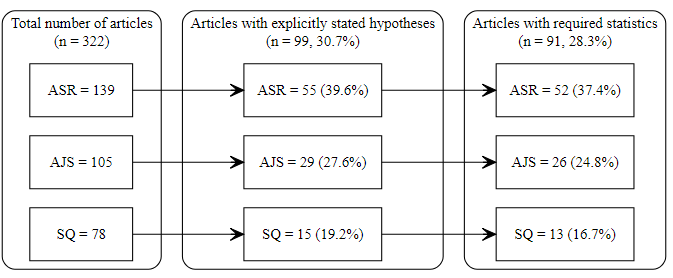
\includegraphics{Flowchart_thesis.png}
\caption{Flowchart describing the process of selecting articles from
which results were retrieved for `Hyp'.}
\end{figure}

~~~~There are some differences between our study on publication bias and
that of Gerber \& Malhotra (2008). Gerber \& Malhotra (2008) performed
caliper tests on \emph{z}-values and \emph{t}-values (converted to
\emph{z}-values) within 5\%, 10\%, 15\%, or 20\% of \emph{z} = 1.64
(one-sided testing) and \emph{z} = 1.96 (two-sided testing). If
\emph{z}-values or \emph{t}-values were unavailable, regression
coefficients and standard errors were used to calculate \emph{z}-values.
We used only exactly reported (not recalculated) \emph{p}-values in the
intervals (.04-.06{]} and (.03-.07{]} to study publication bias
instead.\footnote{It should be noted that these \emph{p}-value intervals
  largely overlap with the 5\% and 10\% caliper tests of Gerber \&
  Malhotra (2008). E.g., for two-sided tests, the 5\% caliper had an
  equivalent \emph{p}-value interval of (.039-.063), while the 10\%
  caliper had an equivalent \emph{p}-value interval of (.031-.077{]}.}
We did this because it was often unknown what kind of distribution an
analysis was based on, and because it allowed us to also include
\emph{p}-values based on \emph{F}-values, \emph{r}-values, and
\(\chi^2\)-values. We did not mix reported and recalculated
\emph{p}-values in our analyses because Krawczyk (2015) and Hartgerink
et al. (2016) found that there can be differences in reported and
recalculated \emph{p}-value distributions around \emph{p} = .05, and
Hartgerink et al. (2016) have argued that these two types of
\emph{p}-values should therefore not be mixed in studies on reporting
practices. Finally, Gerber \& Malhotra (2008) excluded articles with
more than 38 relevant coefficients because their inclusion could have a
disproportionate impact on analyses. We did not do so since we wanted to
include all \emph{p}-values relevant for studying publication bias.\\
\hspace*{0.333em}\hspace*{0.333em}\hspace*{0.333em}\hspace*{0.333em}We
organized all available aspects of a result of an explicitly stated
hypothesis - \emph{p}-value, regression coefficient (or odds ratio,
proportional hazard, etc.), \emph{z}-value, \emph{t}-value,
\emph{F}-value, \emph{r}-value, \(\chi^2\)-value, standard error, sample
size, \emph{df}, phrasing of the hypothesis a result belonged to as
retrieved from the article, and, if applicable, text from the article in
which a result was mentioned - as we did for `APA'. In total, `Hyp'
contained 4,929 results (see Table 1). It was used to study all our
results-related phenomena of interest (see Table 2). Where possible, we
checked whether statistical results were (grossly) inconsistent by
recalculating their \emph{p}-values using the following functions from
the R stats package (R Core Team, 2013): pt() for \emph{t}-values and
\emph{r}-values\footnote{In order to use the pt() function on
  \emph{r}-values, \emph{r}-values first had to be converted to
  \emph{t}-values with the formula:
  \[ t = \frac{r\sqrt{df}}{\sqrt{1-r^2}} \] where \emph{df} = \emph{n} -
  2.}, pnorm() for \emph{z}-values, pf() for \emph{F}-values, and
pchisq() for \(\chi^2\)-values. For detailed information on how this was
done, see Table 3 and Table 4. We also manually added information to
`Hyp' on assignment of marginal significance to in-text \emph{p}-values
in the (.05-.10{]} interval as we did for `AllP'. For \emph{p}-values in
captions of tables and figures, we considered significance levels of
\emph{p} \textless{} .10 (indicated by, e.g., an asterisk) to be
assignment of marginal significance. Finally, among articles in `Hyp'
with \emph{p}-values in the interval (.05-.10{]}, we studied the
percentage of articles in which marginal significance was assigned at
least once to a \emph{p}-value in this interval. Note that `AllP',
`APA', and `Hyp' overlap. For instance, an in-text APA-reported result
related to an explicitly stated hypothesis is included in all three data
sets.\\

\begin{table}[H]

\caption{\label{tab:Table 3 definition consistencies and gross inconsistencies Hyp}Inconsistencies and gross inconsistencies as determined for different types of reported p-values in  ‘Hyp'.}
\centering
\fontsize{12}{14}\selectfont
\begin{tabular}[t]{ccc}
\toprule
Type of Rep\emph{P} & Inconsistent if... & Grossly inconsistent if...\\
\midrule
ns & Cal\emph{P} $\leq$ .05 & Cal\emph{P} $\leq$ .05\\
$<$ & Cal\emph{P} $\geq$ Rep\emph{P} & Cal\emph{P} $>$ .05 \& Rep\emph{P} $\leq$ .05\\
$\geq$ & Cal\emph{P} $<$ Rep\emph{P} & Cal\emph{P} $<$ .05 \& Rep\emph{P} $\geq$ .05\\
= & Cal\emph{P} $\neq$ Rep\emph{P} not due to & Cal\emph{P} $\neq$ Rep\emph{P} not due to rounding,\\
 & rounding\textsuperscript{*} & Cal\emph{P} $\leq$ .05 \& Rep\emph{P} $>$ .05 or vice versa\\
\bottomrule
\multicolumn{3}{l}{\textsuperscript{} \emph{Note}. Cal\emph{P} = recalculated \emph{p}-value, Rep\emph{P} = reported \emph{p}-value, ns = non-significant}\\
\multicolumn{3}{l}{\textsuperscript{*} See Table 4 for methods used to determine whether a difference between recalculated and}\\
\multicolumn{3}{l}{\textsuperscript{} reported \emph{p}-values could be due to correct rounding or not.}\\
\end{tabular}
\end{table}
\pagebreak

\begingroup\fontsize{12}{14}\selectfont

\begin{longtable}[t]{l}
\caption{\label{tab:Table 4 difference exactly reported and recalculated p-values (not) due to rounding}Ways of determining whether discrepancies between exactly reported p-values and their recalculated counterparts from  ‘Hyp' could be due to correct rounding or indicate an inconsistency.}\hspace{1em}\hspace{1em}\\
\toprule
\endfirsthead
\caption[]{Ways of determining whether discrepancies between exactly reported p-values and their recalculated counterparts from  ‘Hyp' could be due to correct rounding or indicate an inconsistency. \textit{(continued)}}\\
\toprule
\endhead

\endfoot
\bottomrule
\multicolumn{1}{l}{\rule{0pt}{1em}\emph{Note}. Rep\emph{P} = reported \emph{p}-value, Cal\emph{P} = recalculated \emph{p}-value, Cal\emph{P}\textsubscript{lb} = lower bound}\\
\multicolumn{1}{l}{\rule{0pt}{1em}recalculated \emph{p}-value, Cal\emph{P}\textsubscript{ub} = upper bound recalculated \emph{p}-value, \emph{b}\textsubscript{lb} = lower bound \emph{b}}\\
\multicolumn{1}{l}{\rule{0pt}{1em}\emph{b}\textsubscript{ub} = upper bound \emph{b}, SE\textsubscript{lb} = lower bound SE, SE\textsubscript{ub} = upper bound SE.}\\
\endlastfoot
\addlinespace[0.3em]
\multicolumn{1}{l}{\textbf{b \& SE}}\\
\hspace{1em}Only used for recalculation if a result was explicitly based on the \emph{z}-distribution or\\
\hspace{1em}\emph{t}-distribution. Take, e.g., \emph{b} $=$ 3.11, SE $=$ 2.11, \emph{p} $=$ 0.07, from a \emph{z}-distribution:\\
\hspace{1em}\hspace{1em}- Correct Cal\emph{P} stem from \emph{b}\textsubscript{lb} $\leq$ \emph{b} $<$ \emph{b}\textsubscript{ub} (e.g., 3.105 $\leq$ \emph{b} $<$ 3.115) and\\
\hspace{1em}\hspace{1em}SE\textsubscript{lb} $\leq$ SE $<$ SE\textsubscript{ub} (e.g., 2.105 $\leq$ SE $<$ 2.115).\\
\hspace{1em}\hspace{1em}- Calculate \emph{t}/\emph{z}\textsubscript{ub} $=$ $\frac{\emph{b} \textsubscript{ub}}{SE\textsubscript{lb}}$ and \emph{t}/\emph{z}\textsubscript{lb} $=$ $\frac{\emph{b} \textsubscript{lb}}{SE\textsubscript{ub}}$, the largest and smallest \emph{t}/\emph{z} consistent\\
\hspace{1em}\hspace{1em}with \emph{b} and SE (e.g., \emph{z}\textsubscript{ub} $=$ $\frac{3.115}{2.105}$ $=$ 1.47981 and \emph{z}\textsubscript{lb} $=$ $\frac{3.105}{2.115}$ $=$ 1.468085).\\
\hspace{1em}\hspace{1em}- Calculate \emph{t}/\emph{z}\textsubscript{lb} $=$ Cal\emph{P}\textsubscript{ub} and \emph{t}/\emph{z}\textsubscript{ub} = Cal\emph{P}\textsubscript{lb}, i.e., boundaries of correctly\\
\hspace{1em}\hspace{1em}rounded Rep\emph{P}. For this, the R stats package pt() function (for \emph{t}) or the pnorm()\\
\hspace{1em}\hspace{1em}function (for \emph{z}) is used.\\
\hspace{1em}\hspace{1em}- Round Cal\emph{P}\textsubscript{lb} and Cal\emph{P}\textsubscript{ub} to the same number of decimals as Rep\emph{P} with\\
\hspace{1em}\hspace{1em}R base round() function. In our example, Cal\emph{P}\textsubscript{lb} $\approx$ 0.07 and Cal\emph{P}\textsubscript{ub} $\approx$ 0.07.\\
\hspace{1em}\hspace{1em}- If Cal\emph{P}\textsubscript{lb} $\leq$ Rep\emph{P} $\leq$ Cal\emph{P}\textsubscript{ub}, Rep\emph{P} is considered correct. This is the case in our\\
\hspace{1em}\hspace{1em}example.\\
\\
\addlinespace[0.3em]
\multicolumn{1}{l}{\textbf{test statistics}}\\
\hspace{1em}Functions of the R stats package used to recalculate \emph{p}-values: pt() for \emph{t} and \emph{r},\\
\hspace{1em}pnorm() for \emph{z}, pf() for \emph{F}, and chisq() for $\chi^2$. All functions, except pnorm(), require \emph{df}.\\
\hspace{1em}We use the example of \emph{t}(61) $=$ 3.11, \emph{p} $=$ 0.0001:\\
\hspace{1em}\hspace{1em}- Correct Cal\emph{P} stem from \emph{t}\textsubscript{lb} $\leq$ \emph{t} $<$ \emph{t}\textsubscript{ub} (e.g., 3.105 $\leq$ \emph{t} $<$ 3.115).\\
\hspace{1em}\hspace{1em}-   Calculate Cal\emph{P}\textsubscript{lb} and Cal\emph{P}\textsubscript{ub}, i.e., the \emph{p}-values consistent with the highest and\\
\hspace{1em}\hspace{1em}lowest \emph{t}-values possible under correct rounding, using pt() function.\\
\hspace{1em}\hspace{1em}- Round Cal\emph{P}\textsubscript{lb} and Cal\emph{P}\textsubscript{ub} to the same number of decimals as Rep\emph{P} with R base\\
\hspace{1em}\hspace{1em}round() function. In our example, Cal\emph{P}\textsubscript{lb} $\approx$ 0.001 and Cal\emph{P}\textsubscript{ub} $\approx$ 0.001.\\
\hspace{1em}\hspace{1em}- If Cal\emph{P}\textsubscript{lb} $\leq$ Rep\emph{P} $\leq$ Cal\emph{P}\textsubscript{ub}, Rep\emph{P} is considered correct. This is not the case in\\
\hspace{1em}\hspace{1em}our example, since Rep\emph{P} $<$ Cal\emph{P}\textsubscript{lb} $<$ Cal\emph{P}\textsubscript{ub}.\\*
\end{longtable}
\endgroup{}

\hypertarget{statistical-analyses}{%
\subsection{Statistical analyses}\label{statistical-analyses}}

In our descriptive analyses (which consist of frequencies and
percentages), we reported how many journals from `SRG' require authors
to adhere to the APA statistical reporting guidelines. For (gross)
inconsistencies, descriptive statistics were based on reproducible
results from `APA' and `Hyp'. We followed Vermeulen et al. (2015) and
Nuijten et al. (2016) by studying the direction of gross
inconsistencies: do errors make non-significant results significant, or
vice versa? For publication bias and the `bump' in \emph{p}-values,
descriptive results were based on exactly reported \emph{p}-values from
`AllP' and `Hyp'. Inexactly reported \emph{p}-values were excluded for
these topics because, as Hartgerink et al. (2016) has shown for a `bump'
in \emph{p}-values, they can lead to `spikes' in certain \emph{p}-values
(e.g., including \emph{p} \textless{} .05 will likely lead to a spike at
\emph{p} = .05). Data sets `AllP' and `Hyp' also provided descriptive
statistics at the results and article level for marginal significance.
For all topics but statistical reporting guidelines, descriptive results
were split by explicitly stated hypothesis (yes/no), journal
(\emph{ASR}, \emph{AJS}, \emph{SQ}, and, for results from `APA' and
`AllP', \emph{CHQ}, and \emph{JMF}), and year (2014-2016).\\
\hspace*{0.333em}\hspace*{0.333em}\hspace*{0.333em}\hspace*{0.333em}Nuijten
et al. (2017) have argued that the prevalence of (gross) inconsistencies
can be studied in three ways. Firstly, one can calculate the percentages
of inconsistencies and gross inconsistencies for each article and take
the averages of these percentages over all articles. Secondly, one can
calculate the overall percentage of (gross) inconsistencies by dividing
the amount of (gross) inconsistencies by the total number of obtained
reported results. This is what we have done in our descriptive analyses.
Finally, Nuijten et al. (2017) described that one can use multilevel
logistic regression models to estimate the probability that a reported
result is inconsistent, while controlling for the nesting of results
within articles. Although this method is in theory statistically sound
or even recommended, simulation analyses revealed that it performs
poorly; because both the number of results per article and the
probability of a gross inconsistency were too low, it was accompanied by
a too low Type I error, a lack of statistical power, and inaccurate
effect size estimates (Nuijten et al., 2017). Therefore, following
Wicherts et al. (2011) and Nuijten et al. (2016), we tested our
hypotheses on statistical reporting errors (H1 and H2) using standard
logistic regressions.~\\
\hspace*{0.333em}\hspace*{0.333em}\hspace*{0.333em}\hspace*{0.333em}We
also conducted logistic regressions to test our hypotheses on
publication bias (H3a, H3b) with exactly reported \emph{p}-values from
`AllP' as the dependent variable. Since statcheck interprets results
with \emph{p} = .05 as being statistically significant (Epskamp \&
Nuijten, 2016), \emph{p} = .05 was included in the interval of just
significant \emph{p}-values for the logistic regressions. To test our
hypothesis on \emph{p}-values reported as marginally significant (H4),
we conducted logistic regressions with exactly reported \emph{p}-values
in the interval (.05-.10{]} from `AllP' as the dependent variable. All
logistic regression analyses contained a binary predictor indicating
whether a result was related to an explicitly stated hypothesis or not.
We chose not to include other potentially relevant control variables,
such as journal and year of publication, because some analyses had too
little data for including multiple predictors.

\vspace{2cm}

\hypertarget{results}{%
\section{Results}\label{results}}

In this section, we start by presenting our results regarding
statistical reporting guidelines. Next, results on statistical reporting
errors, publication bias, the `bump' in \emph{p}-values, and marginal
significance are discussed. For each results-related topic, we first
present automatically retrieved descriptive results and (if applicable)
results of hypothesis testing. Then, we discuss descriptive statistics
of results related to explicitly stated hypotheses from `Hyp'. Results
on specific years and journals that were of little theoretical interest
or were based on too little data are not discussed in the text but can
be found in the corresponding tables.\\

\hypertarget{statistical-reporting-guidelines}{%
\subsection{Statistical reporting
guidelines}\label{statistical-reporting-guidelines}}

Of the 143 sociology journals in `SRG', one journal (\emph{Society}) did
not seem to have any guidelines authors are explicitly required or
allowed to follow when preparing their manuscripts. Four journals
(2.8\%) explicitly required authors to follow guidelines established by
the journal itself, and 102 (71.3\%) required authors to adhere to
(reference) guidelines established by external organizations. Only 13
journals (9.1\%) requested authors to adhere to the APA manual, and
thereby, to the APA statistical reporting guidelines. See Table 5 for an
overview of statistics on sociology journals requesting/allowing
adherence to different statistical reporting guidelines. \pagebreak

\begin{table}[H]

\caption{\label{tab:Table 5 statistical reporting guidelines}Numbers and percentages of sociology journals in ‘SRG' requesting/allowing adherence to different types of statistical reporting guidelines.}
\centering
\fontsize{10}{12}\selectfont
\begin{threeparttable}
\begin{tabular}[t]{lc}
\toprule
  & Number of journals (\% of total)\\
\midrule
\addlinespace[0.3em]
\multicolumn{2}{l}{\textbf{Required}}\\
\hspace{1em}APA & \\
\hspace{1em}\hspace{1em}Full manual & 10 (7\%)\\
\hspace{1em}\hspace{1em}Only references & 10 (7\%)\\
\hspace{1em}ASA & \\
\hspace{1em}\hspace{1em}Full manual & 12 (8.4\%)\\
\hspace{1em}\hspace{1em}Only references & 3 (2.1\%)\\
\hspace{1em}Chicago & \\
\hspace{1em}\hspace{1em}Full manual & 7 (4.9\%)\\
\hspace{1em}\hspace{1em}Only references & 6 (4.2\%)\\
\hspace{1em}Harvard & \\
\hspace{1em}\hspace{1em}Full manual & 2 (1.4\%)\\
\hspace{1em}\hspace{1em}Only references & 9 (6.3\%)\\
\hspace{1em}Oxford & 1 (0.7\%)\\
\hspace{1em}Style Manual for Authors, Editors and Printers & 1 (0.7\%)\\
\hspace{1em}Other & 34 (23.8\%)\\
\hspace{1em}Own & 4 (2.8\%)\\
\hspace{1em}Multiple required & 37 (25.9\%)\\
\hspace{1em}Multiple required (one is full APA manual) & 3 (2.1\%)\\
\hspace{1em}Multiple options (one must be chosen) & 2 (1.4\%)\\
\addlinespace[0.3em]
\multicolumn{2}{l}{\textbf{Other, namely...}}\\
\hspace{1em}Multiple allowed & 1 (0.7\%)\\
\hspace{1em}Unknown* & 1 (0.7\%)\\
\hspace{1em}Total & 143 (100\%)\\
\bottomrule
\end{tabular}
\begin{tablenotes}[para]
\item[*] We were unable to find which guidelines authors publishing in the journal \emph{Society} are required or allowed to use. The link on the journal's website that should have provided access to this information gave a ‘page not found’ error.
\end{tablenotes}
\end{threeparttable}
\end{table}

\hypertarget{statistical-reporting-errors}{%
\subsection{Statistical reporting
errors}\label{statistical-reporting-errors}}

Of the 505 `APA' results, 69 (13.7\%) were inconsistent and 8 (1.6\%)
grossly inconsistent (see Table 6). All grossly inconsistent results had
a statistically significant reported \emph{p}-value and a
non-significant recalculated \emph{p}-value. Out of 168 results related
to explicitly stated hypotheses, 22 (13.1\%) were inconsistent and 4
(2.4\%) grossly inconsistent. Out of 337 results not related to
explicitly stated hypotheses, 47 (13.9\%) were inconsistent and 4
(1.2\%) grossly inconsistent. Of the recalculated \emph{p}-values from
`APA', 416 (82.4\%) were retrieved from the two APA journals. These
journals, \emph{JMF} and \emph{CHQ}, had comparable percentages of
inconsistencies (14.6\% and 14.7\%, respectively) and gross
inconsistencies (1.6\% and 1.7\%, respectively). We found a lower
prevalence of inconsistencies among automatically retrieved results for
non-APA journals \emph{ASR} and \emph{AJS} (2.3\% and 4.9\%,
respectively). Our hypotheses that less (gross) inconsistencies would be
observed for results of explicitly stated hypotheses were not confirmed.
As for H1, the odds of a result of an explicitly stated hypothesis being
inconsistent were \(\frac{1}{.930} \approx 1.076\) times smaller than
the odds that a result not related to an explicitly stated hypothesis
was inconsistent, \emph{b} = -.073, \emph{p} = .793, OR = .930, 95\% CI
{[}.531, 1.585{]}. Regarding H2, the odds of a result of an explicitly
stated hypothesis being grossly inconsistent were 2.030 two times larger
than the odds that a result not related to an explicitly stated
hypothesis was grossly inconsistent, but this difference was not
statistically significant, \emph{b} = .708, \emph{p} = .321, OR = 2.030,
95\% CI {[}.475, 8.685{]}. Full results of the logistic regressions used
to test H1 and H2 can be found in Table S1. Among recalculated
\emph{p}-values from `Hyp', 14 out of 404 were inconsistent (3.5\%), and
2 (0.5\%) were grossly inconsistent. Again, the grossly inconsistent
results had a statistically significant reported \emph{p}-value and a
nonsignificant recalculated \emph{p}-value. For a comprehensive overview
of statistical reporting errors at the article and results level, see
Table S2.

\begin{longtable}[t]{lcccc}
\caption{\label{tab:Table 6 statistical reporting errors}Descriptive statistics on (gross) inconsistencies for ‘APA' and ‘Hyp'.}\\
\toprule
  & Articles & Results & Inconsistencies & Gross inconsistencies\\
\midrule
\endfirsthead
\caption[]{Descriptive statistics on (gross) inconsistencies for ‘APA' and ‘Hyp'. \textit{(continued)}}\\
\toprule
  & Articles & Results & Inconsistencies & Gross inconsistencies\\
\midrule
\endhead

\endfoot
\bottomrule
\endlastfoot
\addlinespace[0.3em]
\multicolumn{5}{l}{\textbf{‘APA'}}\\
\cellcolor{gray!6}{\hspace{1em}Relation to hypothesis} & \cellcolor{gray!6}{} & \cellcolor{gray!6}{} & \cellcolor{gray!6}{} & \cellcolor{gray!6}{}\\
\hspace{1em}\hspace{1em}Yes &  & 168 & 22 (13.1\%) & 4 (2.4\%)\\
\cellcolor{gray!6}{\hspace{1em}\hspace{1em}No} & \cellcolor{gray!6}{} & \cellcolor{gray!6}{337} & \cellcolor{gray!6}{47 (13.9\%)} & \cellcolor{gray!6}{4 (1.2\%)}\\
\hspace{1em}Journal &  &  &  \vphantom{1} & \\
\cellcolor{gray!6}{\hspace{1em}\hspace{1em}ASR} & \cellcolor{gray!6}{7} & \cellcolor{gray!6}{43} & \cellcolor{gray!6}{1 (2.3\%)} & \cellcolor{gray!6}{1 (2.3\%)}\\
\hspace{1em}\hspace{1em}AJS & 3 & 41 & 2 (4.9\%) & 0 (0\%)\\
\cellcolor{gray!6}{\hspace{1em}\hspace{1em}SQ} & \cellcolor{gray!6}{2} & \cellcolor{gray!6}{5} & \cellcolor{gray!6}{5 (100\%)} & \cellcolor{gray!6}{0 (0\%)}\\
\hspace{1em}\hspace{1em}JMF & 36 & 185 & 27 (14.6\%) & 3 (1.6\%)\\
\cellcolor{gray!6}{\hspace{1em}\hspace{1em}CHQ} & \cellcolor{gray!6}{28} & \cellcolor{gray!6}{231} & \cellcolor{gray!6}{34 (14.7\%)} & \cellcolor{gray!6}{4 (1.7\%)}\\
\hspace{1em}Year &  &  &  \vphantom{1} & \\
\cellcolor{gray!6}{\hspace{1em}\hspace{1em}2014} & \cellcolor{gray!6}{20} & \cellcolor{gray!6}{172} & \cellcolor{gray!6}{22 (12.8\%)} & \cellcolor{gray!6}{1 (0.6\%)}\\
\hspace{1em}\hspace{1em}2015 & 21 & 136 & 15 (11\%) & 3 (2.2\%)\\
\cellcolor{gray!6}{\hspace{1em}\hspace{1em}2016} & \cellcolor{gray!6}{35} & \cellcolor{gray!6}{197} & \cellcolor{gray!6}{32 (16.2\%)} & \cellcolor{gray!6}{4 (2\%)}\\
\hspace{1em}Total & 76 & 505 & 69 (13.7\%) & 8 (1.6\%)\\
\addlinespace[0.3em]
\multicolumn{5}{l}{\textbf{‘Hyp'}}\\
\cellcolor{gray!6}{\hspace{1em}Journal} & \cellcolor{gray!6}{} & \cellcolor{gray!6}{} & \cellcolor{gray!6}{} & \cellcolor{gray!6}{}\\
\hspace{1em}\hspace{1em}ASR & 10 & 331 & 11 (3.3\%) & 1 (0.3\%)\\
\cellcolor{gray!6}{\hspace{1em}\hspace{1em}AJS} & \cellcolor{gray!6}{7} & \cellcolor{gray!6}{68} & \cellcolor{gray!6}{1 (1.5\%)} & \cellcolor{gray!6}{1 (1.5\%)}\\
\hspace{1em}\hspace{1em}SQ & 2 & 5 & 2 (40.0\%) & 0 (0\%)\\
\cellcolor{gray!6}{\hspace{1em}Year} & \cellcolor{gray!6}{} & \cellcolor{gray!6}{} & \cellcolor{gray!6}{} & \cellcolor{gray!6}{}\\
\hspace{1em}\hspace{1em}2014 & 11 & 312 & 11 (3.5\%) & 1 (0.3\%)\\
\cellcolor{gray!6}{\hspace{1em}\hspace{1em}2015} & \cellcolor{gray!6}{3} & \cellcolor{gray!6}{33} & \cellcolor{gray!6}{0 (0\%)} & \cellcolor{gray!6}{0 (0\%)}\\
\hspace{1em}\hspace{1em}2016 & 5 & 59 & 3 (5.1\%) & 1 (1.7\%)\\
\cellcolor{gray!6}{\hspace{1em}Total} & \cellcolor{gray!6}{19} & \cellcolor{gray!6}{404} & \cellcolor{gray!6}{14 (3.5\%)} & \cellcolor{gray!6}{2 (0.5\%)}\\*
\end{longtable}

\hypertarget{publication-bias}{%
\subsection{Publication bias}\label{publication-bias}}

In `AllP', there was no evidence of publication bias. Overall, for
binwidth .01, 32 out of 73 results were just significant (43.8\%), and
for binwidth .02, 64 out of 127 results were just significant (50.4\%)
(see Table 7 and Figures 2.1A and 2.1B). Splitting data among results
not related to hypotheses (Figures 2.2A and 2.2B) and results that were
related to hypotheses (Figures 2.3A and 2.3B), percentages were also
around 50. Hence, we could not reject H\textsubscript{0} for our
hypotheses on publication bias (H3a and H3b). For H3a, there were
\(\frac{1}{.877} \approx 1.140\) times less just significant
\emph{p}-values among results of explicitly stated hypotheses than among
results not related to explicitly stated hypotheses for binwidth .01,
\emph{b} = -.132, \emph{p} = .794, OR = .877, 95\% CI {[}.321, 2.345{]}.
In case of H3b for binwidth .02, H\textsubscript{0} could not be
rejected either, since \emph{b} = -.251, \emph{p} = .521, OR = .778,
95\% CI {[}.358, 1.674{]} (full results of the logistic regressions used
to test H3a and H3b can be found in Table S3). Similarly, for `Hyp', no
evidence of publication bias was found among results related to
explicitly stated hypotheses; we found (slightly) more just significant
\emph{p}-values than just nonsignificant ones, namely 9 out of 14
results (64.3\%) for binwidth .01, and 14 out of 26 (53.8\%) for
binwidth .02 (see Figure 3 and Table 7).

\begin{figure}
\centering
\includegraphics{thesis_files/figure-latex/plots publication bias/bump in p-values AllP-1.pdf}
\caption{Histograms with binwidths .01 and .02 of exactly reported
p-values in the range {[}.01-.11{]} from `AllP'. Information is provided
for the totals of exactly reported p-values, and for exactly reported
p-values (not) related to explicitly stated hypotheses.}
\end{figure}

\begin{figure}
\centering
\includegraphics{thesis_files/figure-latex/plots publication bias/bump in p-values Hyp-1.pdf}
\caption{Histograms with binwidths .01 (3A) and .02 (3B) of exactly
reported p-values related to explicitly stated hypotheses in the range
{[}.01-.11{]} from `Hyp'.}
\end{figure}

\clearpage
\begin{table}[H]

\caption{\label{tab:Table 7 publication bias}Descriptive statistics on publication bias among reported p-values for ‘AllP’ and ‘Hyp’.}
\centering
\fontsize{10}{12}\selectfont
\begin{tabular}[t]{lcc>{\centering\arraybackslash}p{5em}>{\centering\arraybackslash}p{5em}>{\centering\arraybackslash}p{5em}c}
\toprule
\multicolumn{1}{c}{ } & \multicolumn{3}{c}{Binwidth .01} & \multicolumn{3}{c}{Binwidth .02} \\
\cmidrule(l{3pt}r{3pt}){2-4} \cmidrule(l{3pt}r{3pt}){5-7}
  & (.04-.05] & (.05-.06] & Total & (.03-.05] & (.05-.07] & Total\\
\midrule
\addlinespace[0.3em]
\multicolumn{7}{l}{\textbf{‘AllP'}}\\
\hspace{1em}\cellcolor{gray!6}{Relation to hypothesis} & \cellcolor{gray!6}{} & \cellcolor{gray!6}{} & \cellcolor{gray!6}{} & \cellcolor{gray!6}{} & \cellcolor{gray!6}{} & \cellcolor{gray!6}{}\\
\hspace{1em}\hspace{1em}Yes & 10 (41.7\%) & 14 & 24 & 17 (45.9\%) & 20 & 37\\
\hspace{1em}\hspace{1em}\cellcolor{gray!6}{No} & \cellcolor{gray!6}{22 (44.9\%)} & \cellcolor{gray!6}{27} & \cellcolor{gray!6}{49} & \cellcolor{gray!6}{47 (52.2\%)} & \cellcolor{gray!6}{43} & \cellcolor{gray!6}{90}\\
\hspace{1em}Journal &  &  &  &  &  \vphantom{1} & \\
\hspace{1em}\hspace{1em}\cellcolor{gray!6}{ASR} & \cellcolor{gray!6}{8 (40\%)} & \cellcolor{gray!6}{12} & \cellcolor{gray!6}{20} & \cellcolor{gray!6}{11 (37.9\%)} & \cellcolor{gray!6}{18} & \cellcolor{gray!6}{29}\\
\hspace{1em}\hspace{1em}AJS & 3 (42.9\%) & 4 & 7 & 8 (57.1\%) & 6 & 14\\
\hspace{1em}\hspace{1em}\cellcolor{gray!6}{SQ} & \cellcolor{gray!6}{1 (20\%)} & \cellcolor{gray!6}{4} & \cellcolor{gray!6}{5} & \cellcolor{gray!6}{3 (42.9\%)} & \cellcolor{gray!6}{4} & \cellcolor{gray!6}{7}\\
\hspace{1em}\hspace{1em}JMF & 14 (43.8\%) & 18 & 32 & 28 (49.1\%) & 29 & 57\\
\hspace{1em}\hspace{1em}\cellcolor{gray!6}{CHQ} & \cellcolor{gray!6}{6 (66.7\%)} & \cellcolor{gray!6}{3} & \cellcolor{gray!6}{9} & \cellcolor{gray!6}{14 (70\%)} & \cellcolor{gray!6}{6} & \cellcolor{gray!6}{20}\\
\hspace{1em}Year &  &  &  &  &  \vphantom{1} & \\
\hspace{1em}\hspace{1em}\cellcolor{gray!6}{2014} & \cellcolor{gray!6}{13 (44.8\%)} & \cellcolor{gray!6}{16} & \cellcolor{gray!6}{29} & \cellcolor{gray!6}{27 (55.1\%)} & \cellcolor{gray!6}{22} & \cellcolor{gray!6}{49}\\
\hspace{1em}\hspace{1em}2015 & 10 (52.6\%) & 9 & 19 & 20 (52.6\%) & 18 & 38\\
\hspace{1em}\hspace{1em}\cellcolor{gray!6}{2016} & \cellcolor{gray!6}{9 (36\%)} & \cellcolor{gray!6}{16} & \cellcolor{gray!6}{25} & \cellcolor{gray!6}{17 (42.5\%)} & \cellcolor{gray!6}{23} & \cellcolor{gray!6}{40}\\
\hspace{1em}Total & 32 (43.8\%) & 41 & 73 & 64 (50.4\%) & 63 & 127\\
\addlinespace[0.3em]
\multicolumn{7}{l}{\textbf{‘Hyp'}}\\
\hspace{1em}\cellcolor{gray!6}{Journal} & \cellcolor{gray!6}{} & \cellcolor{gray!6}{} & \cellcolor{gray!6}{} & \cellcolor{gray!6}{} & \cellcolor{gray!6}{} & \cellcolor{gray!6}{}\\
\hspace{1em}\hspace{1em}ASR & 2 (40\%) & 3 & 5 & 5 (45.5\%) & 6 & 11\\
\hspace{1em}\hspace{1em}\cellcolor{gray!6}{AJS} & \cellcolor{gray!6}{3 (100\%)} & \cellcolor{gray!6}{0} & \cellcolor{gray!6}{3} & \cellcolor{gray!6}{4 (80\%)} & \cellcolor{gray!6}{1} & \cellcolor{gray!6}{5}\\
\hspace{1em}\hspace{1em}SQ & 4 (66.7\%) & 2 & 6 & 5 (50\%) & 5 & 10\\
\hspace{1em}\cellcolor{gray!6}{Year} & \cellcolor{gray!6}{} & \cellcolor{gray!6}{} & \cellcolor{gray!6}{} & \cellcolor{gray!6}{} & \cellcolor{gray!6}{} & \cellcolor{gray!6}{}\\
\hspace{1em}\hspace{1em}2014 & 4 (66.7\%) & 2 & 6 & 8 (61.5\%) & 5 & 13\\
\hspace{1em}\hspace{1em}\cellcolor{gray!6}{2015} & \cellcolor{gray!6}{1 (50\%)} & \cellcolor{gray!6}{1} & \cellcolor{gray!6}{2} & \cellcolor{gray!6}{1 (50\%)} & \cellcolor{gray!6}{1} & \cellcolor{gray!6}{2}\\
\hspace{1em}\hspace{1em}2016 & 4 (66.7\%) & 2 & 6 & 5 (45.5\%) & 6 & 11\\
\hspace{1em}\cellcolor{gray!6}{Total} & \cellcolor{gray!6}{9 (64.3\%)} & \cellcolor{gray!6}{5} & \cellcolor{gray!6}{14} & \cellcolor{gray!6}{14 (53.8\%)} & \cellcolor{gray!6}{12} & \cellcolor{gray!6}{26}\\
\bottomrule
\end{tabular}
\end{table}

\pagebreak

\hspace{10em}

\hypertarget{bump-in-p-values}{%
\subsection{\texorpdfstring{Bump in
\emph{p}-values}{Bump in p-values}}\label{bump-in-p-values}}

Overall, Table 8, Figure 2, and Figure 3 show no `bump' in
\emph{p}-values in `AllP' or `Hyp'. Using binwidth .01, higher
\emph{p}-value intervals contained 32 out of 64 \emph{p}-values (50\%)
for `AllP' overall (Figure 2.1A), 22 out of 47 (46.8\%) (Figure 2.2A)
for results not related to hypotheses from `AllP', 10 out of 17 (58.8\%)
for results related to hypotheses from `AllP' (Figure 2.3A), and 9 out
of 14 (64.3\%) for results related to hypotheses from `Hyp' (Figure 3A).
Correspondingly, for binwidth .02, the higher \emph{p}-value intervals
contained 64 out of 184 (34.8\%) (Figure 2.1B), 47 out of 133
(35.3\%)(Figure 2.2B), 17 out of 51 (33.3\%) (Figure 2.3B), and 14 out
of 37 (37.8\%) results (Figure 3B), respectively.

\pagebreak

\begin{table}[H]

\caption{\label{tab:Table 8 bump in p-values}Descriptive statistics on the bump in just significant reported p-values for ‘AllP' and ‘Hyp'.}
\centering
\resizebox{\linewidth}{!}{
\begin{tabular}[t]{lcc>{\centering\arraybackslash}p{5em}>{\centering\arraybackslash}p{5em}>{\centering\arraybackslash}p{5em}c}
\toprule
\multicolumn{1}{c}{ } & \multicolumn{3}{c}{Binwidth .01} & \multicolumn{3}{c}{Binwidth .02} \\
\cmidrule(l{3pt}r{3pt}){2-4} \cmidrule(l{3pt}r{3pt}){5-7}
  & (.03-.04] & (.04-.05] & Total & (.01-.03] & (.03-.05] & Total\\
\midrule
\addlinespace[0.3em]
\multicolumn{7}{l}{\textbf{‘AllP'}}\\
\hspace{1em}Relation to hypothesis &  &  &  &  &  & \\
\hspace{1em}\hspace{1em}Yes & 7 & 10 (58.8\%) & 17 & 34 & 17 (33.3\%) & 51\\
\hspace{1em}\hspace{1em}No & 25 & 22 (46.8\%) & 47 & 86 & 47 (35.3\%) & 133\\
\hspace{1em}Journal &  &  &  &  &  \vphantom{1} & \\
\hspace{1em}\hspace{1em}ASR & 3 & 8 (72.7\%) & 11 & 25 & 11 (30.6\%) & 36\\
\hspace{1em}\hspace{1em}AJS & 5 & 3 (37.5\%) & 8 & 23 & 8 (25.8\%) & 31\\
\hspace{1em}\hspace{1em}SQ & 2 & 1 (33.3\%) & 3 & 1 & 3 (75\%) & 4\\
\hspace{1em}\hspace{1em}JMF & 14 & 14 (50\%) & 28 & 44 & 28 (38.9\%) & 72\\
\hspace{1em}\hspace{1em}CHQ & 8 & 6 (42.9\%) & 14 & 27 & 14 (34.1\%) & 41\\
\hspace{1em}Year &  &  &  &  &  \vphantom{1} & \\
\hspace{1em}\hspace{1em}2014 & 14 & 13 (48.1\%) & 27 & 51 & 27 (34.6\%) & 78\\
\hspace{1em}\hspace{1em}2015 & 10 & 10 (50\%) & 20 & 41 & 20 (32.8\%) & 61\\
\hspace{1em}\hspace{1em}2016 & 8 & 9 (52.9\%) & 17 & 28 & 17 (37.8\%) & 45\\
\hspace{1em}Total & 32 & 32 (50\%) & 64 & 120 & 64 (34.8\%) & 184\\
\addlinespace[0.3em]
\multicolumn{7}{l}{\textbf{‘Hyp'}}\\
\hspace{1em}Journal &  &  &  &  &  & \\
\hspace{1em}\hspace{1em}ASR & 3 & 2 (40\%) & 5 & 9 & 5 (35.7\%) & 14\\
\hspace{1em}\hspace{1em}AJS & 1 & 3 (75\%) & 4 & 11 & 4 (26.7\%) & 15\\
\hspace{1em}\hspace{1em}SQ & 1 & 4 (80\%) & 5 & 3 & 5 (62.5\%) & 8\\
\hspace{1em}Year &  &  &  &  &  & \\
\hspace{1em}\hspace{1em}2014 & 4 & 4 (50\%) & 8 & 14 & 8 (36.4\%) & 22\\
\hspace{1em}\hspace{1em}2015 & 0 & 1 (100\%) & 1 & 7 & 1 (12.5\%) & 8\\
\hspace{1em}\hspace{1em}2016 & 1 & 4 (80\%) & 5 & 2 & 5 (71.4\%) & 7\\
\hspace{1em}Total & 5 & 9 (64.3\%) & 14 & 23 & 14 (37.8\%) & 37\\
\bottomrule
\end{tabular}}
\end{table}
\pagebreak

\hypertarget{marginal-significance}{%
\subsection{Marginal significance}\label{marginal-significance}}

In 46 out of 107 articles from `AllP' (43\%) with reported
\emph{p}-values in the interval (.05-.10{]}, at least one \emph{p}-value
in this interval was reported as marginally significant (see Table 9).
Out of 206 `AllP' results with reported \emph{p}-values in the interval
(.05-.10{]}, 72 (35\%) were reported as marginally significant. For
results not related to hypotheses and results related to hypotheses,
this was the case for 52 out of 136 (38.2\%) and 20 out of 70 (28.6\%)
\emph{p}-values in the interval (.05-.10{]}, respectively. Among
journals, the prevalence of \emph{p}-values to which marginal
significance was assigned was highest in \emph{CHQ} (11 out of 21
results, or 52.4\%) and lowest in \emph{AJS} (4 out of 31 results, or
12.9\%). The prevalence of assignment of marginal significance to
\emph{p}-values was comparable between years (33.8\%-35.7\%). Our
hypothesis that assignment of marginal significance is less prevalent
among results related to explicitly stated hypotheses in `AllP' (H4) is
not confirmed, \emph{b} = -.437, \emph{p} = .170, OR = .646, 95\% CI
{[}.342, 1.194{]}. Full results of the logistic regression used to test
H4 can be found in Table S4.\\
\hspace*{0.333em}\hspace*{0.333em}\hspace*{0.333em}\hspace*{0.333em}Table
9 also shows the prevalence of marginal significance in `Hyp'. In 19 of
the 30 articles with \emph{p}-values in the interval (.05-.10{]} from
`Hyp' (63.3\%), at least one \emph{p}-value in this interval was
reported as marginally significant. At the results level, Table 9 shows
that overall, 106 of 130 (81.5\%) \emph{p}-values in the interval
(.05-.10{]} were reported as marginally significant. Reporting results
as marginally significant was most prevalent in \emph{AJS} (72 out of 76
results, or 94.7\%) and least prevalent in \emph{SQ} (5 out of 12
results, or 41.7\%). Among the different years, reporting results as
marginally significant was most prevalent in 2015 (71 out of 74 results,
or 95.9\%) and least prevalent in 2014 (11 out of 24 results, or
45.8\%).\\
\hspace*{0.333em}\hspace*{0.333em}\hspace*{0.333em}\hspace*{0.333em}Interestingly,
the percentage of \emph{p}-values in interval (.05-.10{]} reported as
marginally significant is much higher for manually retrieved statistical
results related to explicitly stated hypotheses in `Hyp' (81.5\%) than
for reported \emph{p}-values in `AllP' (35\%) (\emph{z} = 8.33, \emph{p}
\textless{} .001, \emph{z}-test for two independent proportions).

\begin{longtable}[t]{lcccccc}
\caption{\label{tab:Table 9 marginal significance}Descriptive statistics on marginal significance among reported p-values for ‘AllP’ and ‘Hyp’.}\\
\toprule
\multicolumn{1}{c}{ } & \multicolumn{3}{c}{Article level} & \multicolumn{3}{c}{Results level} \\
\cmidrule(l{3pt}r{3pt}){2-4} \cmidrule(l{3pt}r{3pt}){5-7}
  & Yes & No & Total & Yes & No & Total\\
\midrule
\endfirsthead
\caption[]{Descriptive statistics on marginal significance among reported p-values for ‘AllP’ and ‘Hyp’. \textit{(continued)}}\\
\toprule
  & Yes & No & Total & Yes & No & Total\\
\midrule
\endhead

\endfoot
\bottomrule
\endlastfoot
\addlinespace[0.3em]
\multicolumn{7}{l}{\textbf{‘AllP'}}\\
\hspace{1em}Relation to hypothesis &  &  &  &  &  & \\
\hspace{1em}\hspace{1em}Yes &  &  &  & 20 (28.6\%) & 50 & 70\\
\hspace{1em}\hspace{1em}No &  &  &  & 52 (38.2\%) & 84 & 136\\
\hspace{1em}Journal &  &  &  &  &  \vphantom{1} & \\
\hspace{1em}\hspace{1em}ASR & 11 (44\%) & 14 & 25 & 19 (32.8\%) & 39 & 58\\
\hspace{1em}\hspace{1em}AJS & 3 (20\%) & 12 & 15 & 4 (12.9\%) & 27 & 31\\
\hspace{1em}\hspace{1em}SQ & 3 (37.5\%) & 5 & 8 & 4 (36.4\%) & 7 & 11\\
\hspace{1em}\hspace{1em}JMF & 23 (47.9\%) & 25 & 48 & 34 (40\%) & 51 & 85\\
\hspace{1em}\hspace{1em}CHQ & 6 (54.5\%) & 5 & 11 & 11 (52.4\%) & 10 & 21\\
\hspace{1em}Year &  &  &  &  &  \vphantom{1} & \\
\hspace{1em}\hspace{1em}2014 & 11 (35.5\%) & 20 & 31 & 19 (35.2\%) & 35 & 54\\
\hspace{1em}\hspace{1em}2015 & 17 (44.7\%) & 21 & 38 & 30 (35.7\%) & 54 & 84\\
\hspace{1em}\hspace{1em}2016 & 18 (47.4\%) & 20 & 38 & 23 (33.8\%) & 45 & 68\\
\hspace{1em}Total & 46 (43\%) & 61 & 107 & 72 (35\%) & 134 & 206\\
\addlinespace[0.3em]
\multicolumn{7}{l}{\textbf{‘Hyp'}}\\
\hspace{1em}Journal &  &  &  &  &  & \\
\hspace{1em}\hspace{1em}ASR & 8 (72.7\%) & 3 & 11 & 29 (69\%) & 13 & 42\\
\hspace{1em}\hspace{1em}AJS & 9 (60\%) & 6 & 15 & 72 (94.7\%) & 4 & 76\\
\hspace{1em}\hspace{1em}SQ & 2 (50\%) & 2 & 4 & 5 (41.7\%) & 7 & 12\\
\hspace{1em}Year &  &  &  &  &  & \\
\hspace{1em}\hspace{1em}2014 & 6 (46.2\%) & 7 & 13 & 11 (45.8\%) & 13 & 24\\
\hspace{1em}\hspace{1em}2015 & 6 (85.7\%) & 1 & 7 & 71 (95.9\%) & 3 & 74\\
\hspace{1em}\hspace{1em}2016 & 7 (70\%) & 3 & 10 & 24 (75\%) & 8 & 32\\
\hspace{1em}Total & 19 (63.3\%) & 11 & 30 & 106 (81.5\%) & 24 & 130\\*
\end{longtable}
\vspace{2cm}

\hypertarget{discussion}{%
\section{Discussion}\label{discussion}}

In this article, we studied different aspects of statistical reporting
in sociology. Statistical reporting is of high quality if results are
reproducible and do not contain errors, and if clear communication and
critical evaluation of results within a discipline is possible due to
standardized reporting. We created a data set on reporting guidelines in
sociology with which we studied statistical reporting guidelines of 143
sociology journals. We also created three data sets to study statistical
results reported in sociology articles. These data sets contained either
results retrieved automatically by statcheck from the 2014-2016 volumes
of \emph{ASR}, \emph{AJS}, \emph{SQ}, \emph{JMF}, and \emph{CHQ}, or
manually retrieved results related to explicitly stated hypotheses from
the 2014-2016 volumes of \emph{ASR}, \emph{AJS}, and \emph{SQ}. More
specifically, we studied statistical reporting errors among 505
automatically retrieved APA-reported results and 404 manually retrieved
results related to explicitly stated hypotheses. Furthermore, we studied
publication bias, the `bump' in \emph{p}-values, and marginal
significance among 2,960 automatically retrieved \emph{p}-values and
4,929 manually retrieved \emph{p}-values related to explicitly stated
hypotheses.~\\
\hspace*{0.333em}\hspace*{0.333em}\hspace*{0.333em}\hspace*{0.333em}One
important result of our study is that for all our hypotheses, no
differences between results related to explicitly stated hypotheses and
other results were found. Possibly, sociology authors are not inclined
to report more biased statistical results for explicitly stated
hypotheses. Furthermore, they seemingly do not see the need to `boost'
the evidential value of \emph{p}-values related to hypotheses in the
interval (.05-.10{]} to create an (unwarranted) impression of a true
effect. It should be noted that, in hindsight, we do not see why
inconsistencies that do not change a reported result's statistical
significance would occur more often among results related to hypotheses
than among other results (H1). Instead, a more plausible hypothesis
would be that authors pay more attention to the accuracy of their most
important results. Alternatively, authors could be more precise in
writing down statistically significant results of hypotheses than they
are in writing down non-significant results of hypotheses, since the
former might be more interesting to them due to publication pressure.
Finally, an explanation for not finding differences between results
related to explicitly stated hypotheses and other results is that there
is an actual true effect but that statistical power of our tests was
analyses lacking (505 observations, our largest sample size used for
logistic regressions, is not sufficient to detect small or even medium
true effect sizes). However, our sample statistics also did not hint at
substantial effects of results (not) being related to explicitly stated
hypotheses. ~\\
\hspace*{0.333em}\hspace*{0.333em}\hspace*{0.333em}\hspace*{0.333em}We
found a lack of requested adherence to statistical reporting guidelines
within sociology journals: only 9.1\% required adherence to the APA
statistical reporting guidelines. This is especially troublesome because
none of the other guidelines authors were allowed or required to follow
by sociology journals had statistical reporting guidelines that ensure
reproducibility of results. For this reason, a lack of adherence to the
APA statistical reporting guidelines may hamper reproducibility of
results, which in turn may negatively influence statistical reporting
quality in sociology. Reproducible results can namely be easily assessed
by third parties and may thereby motivate authors to thoroughly check if
their results are reported correctly. Hence, reproducibility of results
could reduce the prevalence of statistical reporting errors. Concretely,
for statistical reporting guidelines to ensure reproducible reporting,
they should require that authors explicitly state for each analysis or
result the test statistic, \emph{df} (if applicable), \emph{p}-value,
and whether the test was one- or two-tailed. All these requirements are
covered by the APA statistical reporting guidelines (see APA, 2022a).~\\
\hspace*{0.333em}\hspace*{0.333em}\hspace*{0.333em}\hspace*{0.333em}We
found that among automatically retrieved statistical APA-reported
results from sociology articles, 13.7\% were inconsistent and 1.6\%
grossly inconsistent. Previous research in psychology found a slightly
lower but comparable prevalence of inconsistencies of 4.3\%-12.8\%
(Bakker \& Wicherts, 2011; Krawczyk, 2015; Nuijten et al., 2016;
Veldkamp et al., 2014; Vermeulen et al., 2015; Wicherts et al., 2011).
The prevalence of gross inconsistencies was comparable to the
0.8\%-2.5\% previously found in psychology (Bakker \& Wicherts, 2011;
Nuijten et al., 2016; Veldkamp et al., 2014; Vermeulen et al., 2015).
Moreover, all gross inconsistencies we found had a significant reported
\emph{p}-value and a nonsignificant recalculated \emph{p}-value. The
phenomenon of there being less significant recalculated \emph{p}-values
than reported ones is in line with research by Vermeulen et al. (2015)
and Nuijten et al. (2016) in psychology. Although these results suggest
that the prevalence and direction of statistical reporting errors is
similar in both fields, we do not know whether these phenomena
generalize to the 11 other APA-journals of sociology. Finally, and
interestingly, we found lower prevalences of inconsistencies among
automatically retrieved results for non-APA journals \emph{ASR} and
\emph{AJS}, suggesting that the absence of APA statistical reporting
guidelines does not seem to negatively impact the prevalence of
statistical reporting errors in sociology. However, we should be careful
interpreting this finding, since these two non-APA-journals are not
representative but are considered top journals in the field. In any
case, as has been suggested for psychology (see Nuijten et al., 2016,
2017), sociology would profit from using statcheck in the review or
editorial phase to prevent statistical reporting errors in the published
literature. ~\\
\hspace*{0.333em}\hspace*{0.333em}\hspace*{0.333em}\hspace*{0.333em}Overall,
we found no evidence of publication bias in sociology. This contrasts
with Gerber \& Malhotra (2008), who did find evidence of publication
bias among results related to explicitly stated hypotheses in
\emph{ASR}, \emph{AJS}, and \emph{SQ}. Of course, it could be that
publication bias was simply not present in the articles we studied, but
difference in methodology may also be at least partially responsible for
the different findings. Gerber \& Malhotra (2008) retrieved
substantially more results because they used reported \emph{z}-values
and \emph{t}-values converted to \emph{z}-values, and they calculated
\emph{z}-values using regression coefficients and standard errors.
Because mixing recalculated and reported \emph{p}-values is not
recommended in analyses of reporting practices (see Hartgerink et al.,
2016), we decided to study only reported \emph{p}-values, resulting in
relatively little data and hence low power to detect publication bias
(if present). However, it is not clear why this different methodology
would affect results of analyses on publication bias. As both direct and
indirect evidence of publication bias in the related field of psychology
is strong (see Lakens, 2015b reevaluation of Masicampo \& Lalande, 2012;
Kühberger et al., 2014), and Gerber and Malhotra (2008) also found
publication bias in sociology, we recommend more research in sociology,
both on the process from conception to submission and acceptance of
articles - as has previously been done in psychology by, e.g., Coursol
\& Wagner (1986) and Franco et al. (2014) - and using more data on
reported statistical results.~\\
\hspace*{0.333em}\hspace*{0.333em}\hspace*{0.333em}\hspace*{0.333em}We
also did not find evidence of a `bump' in \emph{p}-value distributions
of statistical results in sociology. This is in line with our own
expectations and with Hartgerink et al. (2016), who did not find
consistent indications of a `bump' in several psychology journals, and
in accordance with the reanalysis of Masicampo \& Lalande (2012) by
Lakens (2015b). Following Hartgerink et al. (2016), we conclude that the
absence of a `bump' does not say anything, whereas a `bump' suggests the
(extensive) use of \emph{p}-hacking in a field, probably accompanied by
zero or small true effect sizes.~\\
\hspace*{0.333em}\hspace*{0.333em}\hspace*{0.333em}\hspace*{0.333em}Assignment
of marginal significance to \emph{p}-values in the interval (.05-.10{]}
in articles was rather common. Among automatically retrieved results,
its prevalence of 35\% at the results level was somewhat lower than the
almost 40\% found by Ohlsson Collentine et al. (2019) in psychology.
This suggests there is no large systemic difference in the reporting of
marginal significance in both fields. Noteworthy is the much higher
prevalence of marginal significance among manually retrieved results
related to hypotheses (81.5\%). We mainly attribute this difference to
authors being aware that \emph{p}-values in the interval (.05-.10{]} are
of low evidential value, which prevents authors from assigning marginal
significance to these results in the articles' text (Ohlsson Collentine
et al., 2019), whereas assigning marginal significance to these results
in tables and figures may seem less harmful to them. The number of
articles with at least one \emph{p}-value in the interval (.05-.10{]} to
which marginal significance was assigned was also higher among manually
retrieved results related to hypotheses (63.3\%) than among
automatically retrieved results (43\%). Again, this may due to authors
being more wary of assigning marginal significance to in-text
\emph{p}-values in the interval (.05-.10{]}. Generally, in line with
previous findings in psychology (Ohlsson Collentine et al., 2019;
Pritschet et al., 2016), it can be concluded that sociology authors
commonly assign marginal significance to \emph{p}-values in the interval
(.05-.10{]}. ~\\
\hspace*{0.333em}\hspace*{0.333em}\hspace*{0.333em}\hspace*{0.333em}To
conclude, we advise the sociological field to adopt the APA statistical
reporting guidelines or establish its own set of statistical reporting
guidelines. Besides improving reproducibility and the information value
of results, this would enhance standardization, and thus, comparability
of statistical results in sociology, and prevent reporting inconsistent
statistical results by implementing the use of statistical checking
programs such as statcheck. Enforcing statistical reporting guidelines
would also be helpful for meta-research on statistical reporting,
publication bias, and research practices. However, for statistical
reporting guidelines to be most effective, it would be very helpful if
journals and the ASA would actively enforce them. Otherwise, as Krawczyk
(2015) has shown for inexactly reported \emph{p}-values in experimental
psychology APA-journals, suboptimal research practices may still seep
through.\\
~\\

\hypertarget{limitations-suggestions-for-future-research}{%
\subsection{Limitations \& suggestions for future
research}\label{limitations-suggestions-for-future-research}}

Our study has some limitations related to amounts of retrieved data.
Firstly, we retrieved relatively little data on publication bias and the
bump in \emph{p}-values, rendering us unable to provide firm conclusions
on the presence of these phenomena in sociology. This is likely due to
most \emph{p}-values in sociology being reported inexactly and many
results not being reported in-text (also compared to psychology), but in
tables and figures instead. In hindsight, we should have included more
articles to obtain enough data to properly study publication bias and
the `bump' in \emph{p}-values.~\\
\hspace*{0.333em}\hspace*{0.333em}\hspace*{0.333em}\hspace*{0.333em}Methodologically,
there were disadvantages to automatically retrieving data in our study.
As mentioned before, most \emph{p}-values in sociology articles are
reported in tables and can thus only be retrieved manually. Furthermore,
many results are reported in text, but are not APA-reported, rendering
statcheck unable to retrieve them. This was especially the case for the
non-APA journals in our study. Given the tendency to report
\emph{p}-values and statistical results in tables, it is quite likely
that the in-text reported \emph{p}-values and APA-reported results
retrieved by statcheck are a selective set of all reported
\emph{p}-values and APA-reported/reproducible results: they are likely
the most theoretically relevant results reported in a study. This has
consequences for comparisons of our findings to previous studies in
psychology, where it seems to be more common to also report more mundane
\emph{p}-values and APA-reported/reproducible results in text: it is
likely wise not to make one-to-one translations from the parts of our
study using statcheck to studies in psychology that use statcheck.\\
\hspace*{0.333em}\hspace*{0.333em}\hspace*{0.333em}\hspace*{0.333em}
Considering the above, it seems that at present, automatic retrieval
from the text of articles is methodologically not the best way of
collecting data on statistical reporting quality in sociology. Instead,
future research on this topic would ideally focus on retrieving
statistical data from text, tables, and figures. At present, this can
only be done manually, which is a very tedious process. It is therefore
vital for reproductive and meta-analytical research purposes that
software to extract \emph{p}-values and reproducible results from tables
and figures will be developed and/or improved. Only the ability to
automatically extract statistical data from figures and tables will
enable high-quality non-tedious assessment of statistical reporting
quality in sociology. Steps towards automatically extracting data from
figures for meta-analytical purposes have been undertaken in recent
years. Pick et al. (2018), e.g., have developed a promising R package
called metaDigitise, which extracts descriptive statistics such as
standard deviations, means, correlations, and CIs from several
often-used types of plots from articles without major problems. While
metaDigitise does not retrieve all types of individual statistics and
fully reported results from all types of figures, its applicability can
probably be broadened. Automatic data extraction from tables, on the
other hand, seems to have its fair share of problems. In a review
article of proposals for data extraction from the increasingly popular
HTML-tables, Roldán et al. (2020) found that extraction from tables is
inhibited by, e.g., the inability to identify multi-part cells,
context-data cells, and split headers, and the inability to analyze the
structure of a cell's contents. This leads to data extraction only being
possible for certain relatively simple types of tables, which is
suboptimal in a meta-analytical context. Thus, substantial work will
have to be done to enable automatic extraction of statistical data from
tables.\\
\hspace*{0.333em}\hspace*{0.333em}\hspace*{0.333em}\hspace*{0.333em}Finally,
it would certainly be useful for future research to track the progress
made in sociology in implementing statistical reporting guidelines. If
substantial progress is made, it would be interesting to study whether
progress seems to have a positive impact on statistical reporting
quality in sociology. Then, future research can provide recommendations
on how the quality of statistical reporting within sociology could be
improved even more.

\pagebreak

\hypertarget{references}{%
\section{References}\label{references}}

\begingroup

\noindent \vspace{-2em} \setlength{\parindent}{-0.4in}
\setlength{\leftskip}{0.4in} \setlength{\parskip}{7pt}

\hypertarget{refs}{}
\leavevmode\hypertarget{ref-APA_numb_stat_guide}{}%
American Psychological Association. (2022a). \emph{APA style numbers and
statistics guide}.
https://apastyle.apa.org/instructional-aids/numbers-statistics-guide.pdf.

\leavevmode\hypertarget{ref-APA_list_journals}{}%
American Psychological Association. (2022b). \emph{Browse journals by
title}.
\url{https://www.apa.org/pubs/journals/browse?query=Title:*\&type=journal}.

\leavevmode\hypertarget{ref-Armitage}{}%
Armitage, P., McPherson, C. K., \& Rowe, B. C. (1969). Repeated
significance tests on accumulating data. \emph{Psychological Methods},
\emph{132}(2), 235--244. \url{https://doi.org/10.2307/2343787}

\leavevmode\hypertarget{ref-Bakker2011}{}%
Bakker, M., \& Wicherts, J. M. (2011). The (mis)reporting of statistical
results in psychology journals. \emph{Behavior Research Methods},
\emph{43}(3), 666--678. \url{https://doi.org/10.3758/s13428-011-0089-5}

\leavevmode\hypertarget{ref-Bakker2014}{}%
Bakker, M., \& Wicherts, J. M. (2014). Outlier removal and the relation
with reporting errors and quality of psychological research.
\emph{Psychological Methods}, \emph{19}(3), 409--427.
\url{https://doi.org/10.1037/met0000014}

\leavevmode\hypertarget{ref-Benjamin}{}%
Benjamin, D. J., Berger, J. O., Johannesson, M., Nosek, B. A.,
Wagenmakers, E. J., Berk, R., Bollen, K. A., Brembs, B., Brown, L.,
Camerer, C., Cesarini, D., Chambers, C. D., Clyde, M., Cook, T. D.,
Boeck, P. D., Dienes, Z., Dreber, A., Easwaran, K., Efferson, C.,
\ldots{} Johnson, V. E. (2017). Redefine statistical significance.
\emph{Nature Human Behaviour}, \emph{2}(1), 6.
\url{https://doi.org/10.1038/s41562-017-0189-z}

\leavevmode\hypertarget{ref-WOS}{}%
Clarivate Analytics' Web of Science. (2016). \emph{Journal citation
reports: Sociology, 2016}. com.proxy.library.uu.nl/JCRJournalHomeAction.

\leavevmode\hypertarget{ref-Cohen}{}%
Cohen, J. (1992). A power primer. \emph{Psychological Bulletin},
\emph{112}(1), 155--159. \url{https://doi.org/10.1037/14805-018}

\leavevmode\hypertarget{ref-Coursol}{}%
Coursol, A., \& Wagner, E. E. (1986). Effect of positive findings on
submission and acceptance rates. \emph{Professional Psychology: Research
and Practice}, \emph{17}(2), 136--137.
\url{https://doi.org/10.1037/0735-7028.17.2.136}

\leavevmode\hypertarget{ref-DeWinter}{}%
De Winter, J. C. F., \& Dodou, D. (2015). A surge of p-values between
0.041 and 0.049 in recent decades (but negative results are increasing
rapidly too). \emph{PeerJ}, \emph{3}, 1--44.
\url{https://doi.org/10.7717/peerj.73}

\leavevmode\hypertarget{ref-Dickersin}{}%
Dickersin, K. (1990). The existence of publication bias and risk factors
for its occurrence. \emph{Jama}, \emph{263}(10), 1385--1389.
\url{https://doi.org/10.1001/jama.1990.03440100097014}

\leavevmode\hypertarget{ref-Easterbrook}{}%
Easterbrook, P. J., Gopalan, R., Berlin, J. A., \& Matthews, D. R.
(1991). Publication bias in clinical research. \emph{The Lancet},
\emph{337}(8746), 867--872.
\url{https://doi.org/10.1016/0140-6736(91)90201-Y}

\leavevmode\hypertarget{ref-statcheck122}{}%
Epskamp, S., \& Nuijten, M. B. (2016). \emph{Statcheck: Extract
statistics from articles and recompute p values}.
\url{https://cran.r-project.org/src/contrib/Archive/statcheck/}.

\leavevmode\hypertarget{ref-Fanelli2010}{}%
Fanelli, D. (2010). ``Positive'' results increase down the hierarchy of
the sciences. \emph{PloS One}, \emph{5}(4), 1--10.
\url{https://doi.org/10.1371/journal.pone.0010068}

\leavevmode\hypertarget{ref-Fanelli2011}{}%
Fanelli, D. (2011). Negative results are disappearing from most
disciplines and countries. \emph{Scientometrics}, \emph{90}(3),
891--904. \url{https://doi.org/10.1007/s11192-011-0494-7}

\leavevmode\hypertarget{ref-Franco2014}{}%
Franco, A., Malhotra, N., \& Simonovits, G. (2014). Publication bias in
the social sciences: Unlocking the file drawer. \emph{Science},
\emph{6203}(345), 1502--1505.
\url{https://doi.org/10.1126/science.1255484}

\leavevmode\hypertarget{ref-Franco2016}{}%
Franco, A., Malhotra, N., \& Simonovits, G. (2016). Underreporting in
psychology experiments: Evidence from a study registry. \emph{Social
Psychological and Personality Science}, \emph{7}(1), 8--12.
\url{https://doi.org/10.1177/1948550615598377}

\leavevmode\hypertarget{ref-Gerber2006}{}%
Gerber, A. S., \& Malhotra, N. (2006). \emph{Can political science
literatures be believed? A study of publication bias in the APSR and the
AJPS}. Paper presented at the annual meeting of the Midwest Political
Science Association.

\leavevmode\hypertarget{ref-Gerber2008}{}%
Gerber, A. S., \& Malhotra, N. (2008). Publication bias in empirical
sociological research: Do arbitrary significance levels distort
published results? \emph{Sociological Methods and Research},
\emph{37}(1), 3--30. \url{https://doi.org/10.1177/0049124108318973}

\leavevmode\hypertarget{ref-Ginsel}{}%
Ginsel, B., Aggarwal, A., Xuan, W., \& Harris, I. (2015). The
distribution of probability values in medical abstracts: An
observational study. \emph{BMC Research Notes}, \emph{8}(1), 1--5.
\url{https://doi.org/10.1186/s13104-015-1691-x}

\leavevmode\hypertarget{ref-Hartgerink2017}{}%
Hartgerink, C. H. J. (2017). Reanalyzing Head et al. (2015):
Investigating the robustness of widespread p-hac. \emph{PeerJ},
\emph{5}, 1--10. \url{https://doi.org/10.7717/peerj.3068}

\leavevmode\hypertarget{ref-Hartgerink2016}{}%
Hartgerink, C. H. J., Van Aert, R. C. M., Nuijten, M. B., Wicherts, J.
M., \& Van Assen, M. A. L. M. (2016). Distributions of p-values smaller
than. 05 in psychology: What is going on? \emph{PeerJ}, \emph{4}, 1--28.
\url{https://doi.org/10.7717/peerj.1935}

\leavevmode\hypertarget{ref-Head2015}{}%
Head, M. L., Holman, L., Lanfear, R., Khan, A. T., \& Jennions, M. D.
(2015). The extent and consequences of p-hacking in science. \emph{PLoS
Biology}, \emph{13}(3), 1--15.
\url{https://doi.org/10.1371/journal.pbio.1002106}

\leavevmode\hypertarget{ref-John}{}%
John, L. K., Loewenstein, G., \& Prelec, D. (2012). Measuring the
prevalence of questionable research practices with incentives for truth
telling. \emph{Psychological Science}, \emph{23}(5), 524--532.
\url{https://doi.org/10.1177/0956797611430953}

\leavevmode\hypertarget{ref-Knight}{}%
Knight, J. (2003). Negative results: Null and void. \emph{Nature},
\emph{422}(6932), 554--555. \url{https://doi.org/10.1038/422554a}

\leavevmode\hypertarget{ref-Krawczyk}{}%
Krawczyk, M. (2015). The search for significance: A few peculiarities in
the distribution of p values in experimental psychology literature.
\emph{PloS One}, \emph{10}(6), 1--19.
\url{https://doi.org/10.1371/journal.pone.0127872}

\leavevmode\hypertarget{ref-Kuhberger}{}%
Kühberger, A., Fritz, A., \& Scherndl, T. (2014). Publication bias in
psychology: A diagnosis based on the correlation between effect size and
sample size. \emph{PloS One}, \emph{9}(9), 1--8.
\url{https://doi.org/10.1371/journal.pone.0105825}

\leavevmode\hypertarget{ref-Lakens2015a}{}%
Lakens, D. (2015a). On the challenges of drawing conclusions from
p-values just below 0.05. \emph{PeerJ}, \emph{3}, 1--14.
\url{https://doi.org/10.7717/peerj.1142}

\leavevmode\hypertarget{ref-Lakens2015b}{}%
Lakens, D. (2015b). What p-hacking really looks like: A comment on
Masicampo and LaLande (2012). \emph{The Quarterly Journal of
Experimental Psychology}, \emph{68}(4), 829--832.
\url{https://doi.org/10.1080/17470218.2014.982664}

\leavevmode\hypertarget{ref-Lang}{}%
Lang, T. A., \& Altman, D. G. (2013). Basic statistical reporting for
articles published in clinical medical journals: The SAMPL Guidelines.
In P. Smart, H. Maisonneuve, \& A. Polderman (Eds.), \emph{Science
editors' handbook} (pp. 24--30). European Association of Science
Editors.

\leavevmode\hypertarget{ref-Lawrence}{}%
Lawrence, P. A. (2003). The politics of publication - authors, reviewers
and editors must act to protect the quality of research. \emph{Nature},
\emph{422}(6929), 259--261. \url{https://doi.org/10.1038/422259a}

\leavevmode\hypertarget{ref-Leahey}{}%
Leahey, E. (2005). Alphas and asterisks: The development of statistical
significance testing standards in sociology. \emph{Social Forces},
\emph{84}(1), 1--24. \url{https://doi.org/10.1353/sof.2005.0108}

\leavevmode\hypertarget{ref-Leggett}{}%
Leggett, N. C., Thomas, N. A., Loetscher, T., \& Nicholls, M. E. R.
(2013). The life of p: ``Just significant'' results are on the rise.
\emph{The Quarterly Journal of Experimental Psychology}, \emph{66}(12),
2303--2309. \url{https://doi.org/10.1080/17470218.2013.863371}

\leavevmode\hypertarget{ref-Masicampo}{}%
Masicampo, E. J., \& Lalande, D. R. (2012). A peculiar prevalence of p
values just below. 05. \emph{The Quarterly Journal of Experimental
Psychology}, \emph{65}(11), 2271--2279.
\url{https://doi.org/10.1080/17470218.2012.711335}

\leavevmode\hypertarget{ref-Maxwell}{}%
Maxwell, C. (1981). Clinical trials, reviews, and the journal of
negative results. \emph{British Journal of Clinical Pharmacology},
\emph{11}(1), 15--18.
\url{https://doi.org/10.1111/j.1365-2125.1981.tb01095.x}

\leavevmode\hypertarget{ref-Nuijten2017}{}%
Nuijten, M. B., Borghuis, J., Veldkamp, C. L. S., Dominguez Alvarez, L.,
Van Assen, M. A. L. M., \& Wicherts, J. M. (2017). Journal data sharing
policies and statistical reporting inconsistencies in psychology.
\emph{Collabra: Psychology}, \emph{3}(1), 1--22.
\url{https://doi.org/10.1525/collabra.102}

\leavevmode\hypertarget{ref-Nuijten2016}{}%
Nuijten, M. B., Hartgerink, C. H. J., Van Assen, M. A. L. M., Epskamp,
S., \& Wicherts, J. M. (2016). The prevalence of statistical reporting
errors in psychology (1985--2013). \emph{Behavior Research Methods},
\emph{48}(4), 1205--1226.
\url{https://doi.org/10.3758/s13428-015-0664-2}

\leavevmode\hypertarget{ref-OhlssonCollentine}{}%
Ohlsson Collentine, A., Van Assen, M. A. L. M., \& Hartgerink, C. H. J.
(2019). The prevalence of marginally significant results in psychology
over time. \emph{Psychological Science}, \emph{30}(4), 576--586.
\url{https://doi.org/10.1177/0956797619830326}

\leavevmode\hypertarget{ref-Pick}{}%
Pick, J. L., Nakagawa, S., \& Noble, D. W. A. (2018). Reproducible,
flexible and high throughput data extraction from primary literature:
The metaDigitise package. \emph{Methods in Ecology and Evolution},
\emph{10}(3), 426--431. \url{https://doi.org/10.1111/2041-210X.13118}

\leavevmode\hypertarget{ref-Pritschet}{}%
Pritschet, L., Powell, D., \& Horne, Z. (2016). Marginally significant
effects as evidence for hypotheses: Changing attitudes over four
decades. \emph{Psychological Science}, \emph{27}(7), 1036--1042.
\url{https://doi.org/10.1177/0956797616645672}

\leavevmode\hypertarget{ref-Rstats}{}%
R Core Team. (2013). \emph{R: A language and environment for statistical
computing}. R Foundation for Statistical Computing;
\url{http://www.R-project.org/}.

\leavevmode\hypertarget{ref-Roldan}{}%
Roldán, J. C., Jiménez, P., \& Corchuelo, R. (2020). On extracting data
from tables that are encoded using html. \emph{Knowledge-Based Systems},
\emph{190}, 105157. \url{https://doi.org/10.1016/j.knosys.2019.105157}

\leavevmode\hypertarget{ref-Sedlmeier}{}%
Sedlmeier, P., \& Gigerenzer, G. (1989). Do studies of statistical power
have an effect on the power of studies? \emph{Psychological Bulletin},
\emph{105}(2), 309--316. \url{https://doi.org/10.1037/10109-032}

\leavevmode\hypertarget{ref-Simera}{}%
Simera, I., Moher, D., Hirst, A., Hoey, J., Schulz, K. F., \& Altman, D.
G. (2011). Transparent and accurate reporting increases reliability,
utility, and impact of your research: Reporting guidelines and the
EQUATOR Network. \emph{BMC Medicine}, \emph{22}(11), 1359--1366.
\url{https://doi.org/10.1186/1741-7015-8-24}

\leavevmode\hypertarget{ref-Simonsohn}{}%
Simonsohn, U., Nelson, L. D., \& Simmons, J. P. (2014). P-curve: A key
to the file drawer. \emph{Journal of Experimental Psychology: General},
\emph{143}(2), 534--547. \url{https://doi.org/10.1037/a0033242}

\leavevmode\hypertarget{ref-Song}{}%
Song, F., Parekh, S., Hooper, L., Ryder, Y. K., Sutton, A. J., Hing, C.,
Kwok, C. S., Pang, C., \& Harvey, I. (2010). Dissemination and
publication of research findings: An updated review of related biases.
\emph{Health Technology Assessment}, \emph{14}(8), 1--236.
\url{https://doi.org/10.3310/hta14080}

\leavevmode\hypertarget{ref-Ulrich}{}%
Ulrich, R., \& Miller, J. (2015). P-hacking by post hoc selection with
multiple opportunities: Detectability by skewness test?: Comment on
Simonsohn, Nelson, and Simmons (2014). \emph{Journal of Experimental
Psychology: General}, \emph{144}(6), 1137--1145.
\url{https://doi.org/10.1037/xge0000086}

\leavevmode\hypertarget{ref-Veldkamp}{}%
Veldkamp, C. L., Nuijten, M. B., Dominguez-Alvarez, L., Van Assen, M. A.
L. M., \& Wicherts, J. M. (2014). Statistical reporting errors and
collaboration on statistical analyses in psychological science.
\emph{PloS One}, \emph{9}(12), 1--19.
\url{https://doi.org/10.1371/journal.pone.0114876}

\leavevmode\hypertarget{ref-Vermeulen}{}%
Vermeulen, I., Beukeboom, C. J., Batenburg, A., Avramiea, A., Stoyanov,
D., Van de Velde, B., \& Oegema, D. (2015). Blinded by the light: How a
focus on statistical ``significance'' may cause p-value misreporting and
an excess of p-values just below .05 in communication science.
\emph{Communication Methods and Measures}, \emph{9}(4), 253--279.
\url{https://doi.org/10.1080/19312458.2015.1096333}

\leavevmode\hypertarget{ref-Wicherts}{}%
Wicherts, J. M., Bakker, M., \& Molenaar, D. (2011). Willingness to
share research data is related to the strength of the evidence and the
quality of reporting of statistical results. \emph{PloS One},
\emph{6}(11), 1--7. \url{https://doi.org/10.1371/journal.pone.0026828}

.

\endgroup

\newpage

\beginsupplement

\hypertarget{supplement}{%
\section{Supplement}\label{supplement}}

\begin{table}[H]

\caption{\label{tab:Table S1 logistic regressions statistical reporting errors}Logistic regressions for H1 and H2, which concern the difference in prevalence of (gross) inconsistencies in results related to hypotheses versus results not related to hypotheses.}
\centering
\begin{tabular}[t]{lccccc}
\toprule
  & b & SE & z & p & OR [95\% CI]\\
\midrule
\addlinespace[0.3em]
\multicolumn{6}{l}{\textbf{Inconsistencies (H1)}}\\
\cellcolor{gray!6}{\hspace{1em}Intercept} & \cellcolor{gray!6}{-1.820} & \cellcolor{gray!6}{.157} & \cellcolor{gray!6}{-11.573} & \cellcolor{gray!6}{< .001} & \cellcolor{gray!6}{.162 [.118, .218]}\\
\hspace{1em}Result hypothesis & -.073 & .278 & -.262 & .793 & .930 [.531, 1.585]\\
\addlinespace[0.3em]
\multicolumn{6}{l}{\textbf{Gross inconsistencies (H2)}}\\
\cellcolor{gray!6}{\hspace{1em}Intercept} & \cellcolor{gray!6}{-4.422} & \cellcolor{gray!6}{.503} & \cellcolor{gray!6}{-8.791} & \cellcolor{gray!6}{< .001} & \cellcolor{gray!6}{.012 [.004, .028]}\\
\hspace{1em}Result hypothesis & .708 & .714 & .993 & .321 & 2.030 [.475, 8.685]\\
\bottomrule
\end{tabular}
\end{table}

\hspace{20em}
\newline

\begin{table}[H]

\caption{\label{tab:Table S2 statistical reporting errors including results level}Descriptive statistics on (gross) inconsistencies for ‘APA' and ‘Hyp'.}
\centering
\resizebox{\linewidth}{!}{
\begin{tabular}[t]{lcccccc}
\toprule
\multicolumn{1}{c}{ } & \multicolumn{3}{c}{Article level} & \multicolumn{3}{c}{Results level} \\
\cmidrule(l{3pt}r{3pt}){2-4} \cmidrule(l{3pt}r{3pt}){5-7}
  & Total & With inconsistencies & With gross inconsistencies & Total & Inconsistencies & Gross inconsistencies\\
\midrule
\addlinespace[0.3em]
\multicolumn{7}{l}{\textbf{‘APA'}}\\
\cellcolor{gray!6}{\hspace{1em}Relation to hypothesis} & \cellcolor{gray!6}{} & \cellcolor{gray!6}{} & \cellcolor{gray!6}{} & \cellcolor{gray!6}{} & \cellcolor{gray!6}{} & \cellcolor{gray!6}{}\\
\hspace{1em}\hspace{1em}Yes &  &  &  & 168 & 22 (13.1\%) & 4 (2.4\%)\\
\cellcolor{gray!6}{\hspace{1em}\hspace{1em}No} & \cellcolor{gray!6}{} & \cellcolor{gray!6}{} & \cellcolor{gray!6}{} & \cellcolor{gray!6}{337} & \cellcolor{gray!6}{47 (13.9\%)} & \cellcolor{gray!6}{4 (1.2\%)}\\
\hspace{1em}Journal &  &  &  &  &  \vphantom{1} & \\
\cellcolor{gray!6}{\hspace{1em}\hspace{1em}ASR} & \cellcolor{gray!6}{7} & \cellcolor{gray!6}{1 (14.3\%)} & \cellcolor{gray!6}{1 (14.3\%)} & \cellcolor{gray!6}{43} & \cellcolor{gray!6}{1 (2.3\%)} & \cellcolor{gray!6}{1 (2.3\%)}\\
\hspace{1em}\hspace{1em}AJS & 3 & 1 (33.3\%) & 0 (0\%) & 41 & 2 (4.9\%) & 0 (0\%)\\
\cellcolor{gray!6}{\hspace{1em}\hspace{1em}SQ} & \cellcolor{gray!6}{2} & \cellcolor{gray!6}{2 (100\%)} & \cellcolor{gray!6}{0 (0\%)} & \cellcolor{gray!6}{5} & \cellcolor{gray!6}{5 (100\%)} & \cellcolor{gray!6}{0 (0\%)}\\
\hspace{1em}\hspace{1em}JMF & 36 & 12 (33.3\%) & 2 (5.6\%) & 185 & 27 (14.6\%) & 3 (1.6\%)\\
\cellcolor{gray!6}{\hspace{1em}\hspace{1em}CHQ} & \cellcolor{gray!6}{28} & \cellcolor{gray!6}{13 (46.4\%)} & \cellcolor{gray!6}{2 (7.1\%)} & \cellcolor{gray!6}{231} & \cellcolor{gray!6}{34 (14.7\%)} & \cellcolor{gray!6}{4 (1.7\%)}\\
\hspace{1em}Year &  &  &  &  &  \vphantom{1} & \\
\cellcolor{gray!6}{\hspace{1em}\hspace{1em}2014} & \cellcolor{gray!6}{20} & \cellcolor{gray!6}{7 (35\%)} & \cellcolor{gray!6}{1 (5.0\%)} & \cellcolor{gray!6}{172} & \cellcolor{gray!6}{22 (12.8\%)} & \cellcolor{gray!6}{1 (0.6\%)}\\
\hspace{1em}\hspace{1em}2015 & 21 & 7 (33.3\%) & 2 (9.5\%) & 136 & 15 (11.0\%) & 3 (2.2\%)\\
\cellcolor{gray!6}{\hspace{1em}\hspace{1em}2016} & \cellcolor{gray!6}{35} & \cellcolor{gray!6}{15 (42.9\%)} & \cellcolor{gray!6}{2 (5.7\%)} & \cellcolor{gray!6}{197} & \cellcolor{gray!6}{32 (16.2\%)} & \cellcolor{gray!6}{4 (2.0\%)}\\
\hspace{1em}Total & 76 & 29 (38.2\%) & 5 (6.6\%) & 505 & 69 (13.7\%) & 8 (1.6\%)\\
\addlinespace[0.3em]
\multicolumn{7}{l}{\textbf{‘Hyp'}}\\
\cellcolor{gray!6}{\hspace{1em}Journal} & \cellcolor{gray!6}{} & \cellcolor{gray!6}{} & \cellcolor{gray!6}{} & \cellcolor{gray!6}{} & \cellcolor{gray!6}{} & \cellcolor{gray!6}{}\\
\hspace{1em}\hspace{1em}ASR & 10 & 4 (40.0\%) & 1 (10.0\%) & 331 & 11 (3.3\%) & 1 (0.3\%)\\
\cellcolor{gray!6}{\hspace{1em}\hspace{1em}AJS} & \cellcolor{gray!6}{7} & \cellcolor{gray!6}{1 (14.3\%)} & \cellcolor{gray!6}{1 (14.3\%)} & \cellcolor{gray!6}{68} & \cellcolor{gray!6}{1 (1.5\%)} & \cellcolor{gray!6}{1 (1.5\%)}\\
\hspace{1em}\hspace{1em}SQ & 2 & 1 (50.0\%) & 0 (0\%) & 5 & 2 (40.0\%) & 0 (0\%)\\
\cellcolor{gray!6}{\hspace{1em}Year} & \cellcolor{gray!6}{} & \cellcolor{gray!6}{} & \cellcolor{gray!6}{} & \cellcolor{gray!6}{} & \cellcolor{gray!6}{} & \cellcolor{gray!6}{}\\
\hspace{1em}\hspace{1em}2014 & 11 & 4 (36.4\%) & 1 (9.1\%) & 312 & 11 (3.5\%) & 1 (0.3\%)\\
\cellcolor{gray!6}{\hspace{1em}\hspace{1em}2015} & \cellcolor{gray!6}{3} & \cellcolor{gray!6}{0 (0\%)} & \cellcolor{gray!6}{0 (0\%)} & \cellcolor{gray!6}{33} & \cellcolor{gray!6}{0 (0\%)} & \cellcolor{gray!6}{0 (0\%)}\\
\hspace{1em}\hspace{1em}2016 & 5 & 2 (40.0\%) & 1 (20.0\%) & 59 & 3 (5.1\%) & 1 (1.7\%)\\
\cellcolor{gray!6}{\hspace{1em}Total} & \cellcolor{gray!6}{19} & \cellcolor{gray!6}{6 (31.6\%)} & \cellcolor{gray!6}{2 (10.5\%)} & \cellcolor{gray!6}{404} & \cellcolor{gray!6}{14 (3.5\%)} & \cellcolor{gray!6}{2 (0.5\%)}\\
\bottomrule
\end{tabular}}
\end{table}

\hspace{20em}
\newline

\begin{table}[H]

\caption{\label{tab:Table S3 logistic regressions publication bias}Logistic regressions for H3a and H3b, which concerns the difference in prevalence of publication bias in results related to hypotheses versus results not related to hypotheses.}
\centering
\begin{tabular}[t]{lccccc}
\toprule
  & b & SE & z & p & OR [95\% CI]\\
\midrule
\addlinespace[0.3em]
\multicolumn{6}{l}{\textbf{Binwidth .01 (H3a)}}\\
\cellcolor{gray!6}{\hspace{1em}Intercept} & \cellcolor{gray!6}{-.205} & \cellcolor{gray!6}{.287} & \cellcolor{gray!6}{-.713} & \cellcolor{gray!6}{.476} & \cellcolor{gray!6}{.815 [.456, 1.428]}\\
\hspace{1em}Result hypothesis & -.132 & .504 & -.261 & .794 & .877 [.321, 2.345]\\
\addlinespace[0.3em]
\multicolumn{6}{l}{\textbf{Binwidth .02 (H3b)}}\\
\cellcolor{gray!6}{\hspace{1em}Intercept} & \cellcolor{gray!6}{.089} & \cellcolor{gray!6}{.211} & \cellcolor{gray!6}{.421} & \cellcolor{gray!6}{.673} & \cellcolor{gray!6}{1.093 [.723, 1.658]}\\
\hspace{1em}Result hypothesis & -.251 & .392 & -.642 & .521 & .778 [.358, 1.674]\\
\bottomrule
\end{tabular}
\end{table}
\hspace{20em}
\newline

\begin{table}[H]

\caption{\label{tab:Table S4 logistic regression marginal significance}Logistic regression for H4, which concerns the difference in prevalence of marginal significance in results related to hypotheses versus results not related to hypotheses.}
\centering
\begin{tabular}[t]{lccccc}
\toprule
  & b & SE & z & p & OR [95\% CI]\\
\midrule
Intercept & -.480 & .177 & -2.718 & .007 & .619 [.436, .871]\\
Result hypothesis & -.437 & .318 & -1.373 & .170 & .646 [.342, 1.194]\\
\bottomrule
\end{tabular}
\end{table}

\end{document}
